\documentclass{article}

\usepackage[margin=1in]{geometry} % Add this line to set the margins
\usepackage{enumitem}
\usepackage{booktabs}  % For professional looking tables
\usepackage{multirow}
\usepackage{changepage}

\usepackage{caption, amsmath, amsfonts, amssymb, amstext, amscd, amsthm, makeidx, graphicx, hyperref, url, inputenc, float, listings, color, titlesec, indentfirst}
\allowdisplaybreaks

\definecolor{dkgreen}{rgb}{0,0.6,0}
\definecolor{gray}{rgb}{0.5,0.5,0.5}
\definecolor{mauve}{rgb}{0.58,0,0.82}

\lstset{frame=tb,
  language=Java,
  aboveskip=3mm,
  belowskip=3mm,
  showstringspaces=false,
  columns=flexible,
  basicstyle={\small\ttfamily},
  numbers=none,
  numberstyle=\tiny\color{gray},
  keywordstyle=\color{blue},
  commentstyle=\color{dkgreen},
  stringstyle=\color{mauve},
  breaklines=true,
  breakatwhitespace=true,
  tabsize=3
}

\lstset{language=Python}

\titleformat{\paragraph}[runin]{\normalfont\itshape}{\theparagraph}{1em}{}

\pagenumbering{arabic}

\titleformat{\section}
  {\normalfont\Large\bfseries}{\thesection}{1em}{}

\topmargin -1in
\textheight 9.0in

\title{Machine Learning Based Long-Short Strategies on Industry Returns Predictions}
\author{Firdavs Nasriddinov, Manuel Rodriguez}
\date{June 9, 2024}

\begin{document}

\maketitle{}

\section{Abstract}

% This paper investigates the effectiveness of advanced machine learning models, particularly Long Short-Term Memory (LSTM) networks, in predicting financial market trends and generating superior returns. Our strategy involves a comprehensive rolling window approach, where models are trained on historical data from 1926 to the current year and then tested on the subsequent year. This process is repeated annually to assess the models' performance in real-world, dynamic market conditions. We examine various portfolio creation strategies, including Max-Min Long-Short, Weighted Long-Short, and Max Long, to determine the most effective method for leveraging model predictions. Additionally, we benchmark our models against the Capital Asset Pricing Model (CAPM), Fama-French 3-Factor (FF3), and Fama-French 6-Factor (FF6) models to evaluate their relative performance. Our optimal model, an LSTM trained on value-weighted 49 Industry Portfolio Returns with a 5-day lag and employing a Max-Min Long-Short strategy, consistently outperformed other configurations. The LSTM model achieved significant annual alphas of 51.57\% (1980-1995), 17.43\% (1995-2010), and 10.65\% (2010-2020), with corresponding Sharpe ratios of 1.49, 0.40, and 0.38, respectively, indicating robust risk-adjusted returns and minimal correlation with market movements. Our study underscores the importance of model configuration, including the number of industries, input day lags, and portfolio strategy type, in determining performance. Models with a larger number of industries generally outperformed those with fewer industries due to increased diversification. Notably, there was minimal performance difference between 5-day and 22-day lags, suggesting the models can learn effectively with shorter historical data. The Max-Min Long-Short strategy, focusing on the top and bottom deciles of predicted returns, proved crucial for maximizing gains and minimizing risks. This strategy consistently yielded higher alphas and Sharpe ratios compared to other strategies. Overall, our findings demonstrate the significant potential of LSTM models in developing advanced, resilient trading strategies capable of delivering consistent, superior returns across diverse market conditions.

This paper investigates the effectiveness of machine learning models, particularly Long Short-Term Memory (LSTM) networks, in predicting financial market trends and generating large and significant excess returns. Using a rolling window approach, models were trained on historical data from 1926 to the current year and tested on the subsequent year. Various portfolio strategies, including Max-Min Long-Short, Weighted Long-Short, and Max Long, were evaluated, and models were benchmarked against CAPM, FF3, and FF6. The optimal model, an LSTM trained on value-weighted 49 Industry Portfolio Returns with a 5-day lag and a Max-Min Long-Short strategy, consistently outperformed other configurations, achieving significant annual alphas of 51.57\% (1980-1995), 17.43\% (1995-2010), and 10.65\% (2010-2020), with corresponding Sharpe ratios of 1.49, 0.40, and 0.38. This study highlights the importance of model configuration and diversification in achieving high performance and demonstrates the potential of LSTM models in developing advanced trading strategies that deliver consistent, excess returns across diverse market conditions.

\medskip

\section{Introduction}
The hedge fund industry has consistently leveraged a broad array of resources to gain an edge in markets. One of the most recent and transformative applications in this endeavor has been the integration of artificial intelligence and machine learning. The adoption of machine learning techniques has led to a significant evolution in traditional stock arbitrage strategies, which have become less effective. This shift can be attributed to the transition from trading algorithms that relied on human intuition to those that employ highly optimized computational models.

Since the introduction of the Feed Forward Neural Network (FFNN) \cite{ffnn_orig}, these networks have been extensively utilized across various domains due to their capability as universal function approximators. FFNNs have demonstrated substantial utility in finance, as evidenced by numerous studies. Long Short Term Memory (LSTM) networks, a specific type of recurrent neural network, have shown superior performance over FFNNs in tasks such as predicting next-day stock movements \cite{fischer2018} and conducting financial sentiment analysis for stock market predictions \cite{eachempati}. Additionally, Gradient Boosting Decision Trees (GBDT) \cite{boosting-paper} have been explored within the same domain, outperforming FFNNs in predicting next-day stock movements \cite{weng2017} and forecasting daily returns of the S\&P 500 \cite{nevasalmi2020forecasting}.

The primary objective of this is to develop robust trading strategies based on the next-day returns predictions of machine learning models on value-weighted Fama French Industry Portfolio prior lag returns. We implement and compare three distinct models: Feed Forward Neural Networks (FFNN), Long Short-Term Memory (LSTM) networks, and Gradient Boosting Decision Trees (GBDT). Each model is designed to capture different aspects of market behavior and is evaluated on its ability to generate excess returns, or alpha, beyond traditional benchmarks.

Our strategy involves a comprehensive rolling window approach, where models are trained on historical data from 1926 to the current year and then tested on the subsequent year. This process is repeated annually to assess the models' performance in real-world, dynamic market conditions. We examine various portfolio creation strategies, including Max-Min Long-Short, Weighted Long-Short, and Max Long, to determine the most effective method for leveraging model predictions. Additionally, we benchmark our models against the Capital Asset Pricing Model (CAPM), Fama-French 3-Factor (FF3), and Fama-French 5-Factor + Momentum (FF6) models to evaluate their relative performance.

Through this analysis, we aim to identify machine learning models that consistently deliver superior returns across different market regimes, including bullish and bearish periods. Our findings will contribute to the understanding of how advanced computational techniques can enhance trading strategies and potentially improve financial decision-making.

\subsection{Data}
Our strategy was based on trading the value-weighted Fama French Industry Portfolios \cite{french2024}. From {the Fama French website }\cite{FrenchIndustries}, The portfolios are created by "...assign[ing] each NYSE, AMEX, and NASDAQ stock to an industry portfolio at the end of June of year t based on its four-digit SIC code at that time. (We use Compustat SIC codes for the fiscal year ending in calendar year t-1. Whenever Compustat SIC codes are not available, we use CRSP SIC codes for June of year t.) We then compute returns from July of t to June of t+1." An example list of the industries is given in Table 1.

Additionally, we use the Fama French Data Library \cite{french2024} to get the Fama French 3 Factor (FF3) and Fama French 5 Factor + Momentum (FF6) factor returns to compare our models against.
\begin{table}[H]
    \centering
    \begin{tabular}{|c c c c c|}
        Non-Durable Goods & Durable Goods & Manufacturing & Energy & High Technology \\
        Telecommunications & Retail Shops & Health & Utilities & Other 
    \end{tabular}
    \caption{Example of categories: 10-industry portfolio categories.}
    \label{tab:my_label}
\end{table}

\subsection{Models}

\subsubsection{\emph{Feed Forward Neural Network (FFNN)}}
Introduced in the early 1990s \cite{ffnn_orig}, Feed Forward Neural Networks (FFNN) are a foundational architecture in the field of machine learning. These networks consist of an input layer, one or more hidden layers, and an output layer, where the data flows in a single direction from the input to the output. FFNNs are widely used for tasks such as regression and classification due to their simplicity and effectiveness in modeling complex relationships between inputs and outputs. Despite their simplicity, FFNNs serve as a robust baseline model for more complex architectures.

\paragraph{FFNN Structure}
    \begin{figure}[H]
        \centering
        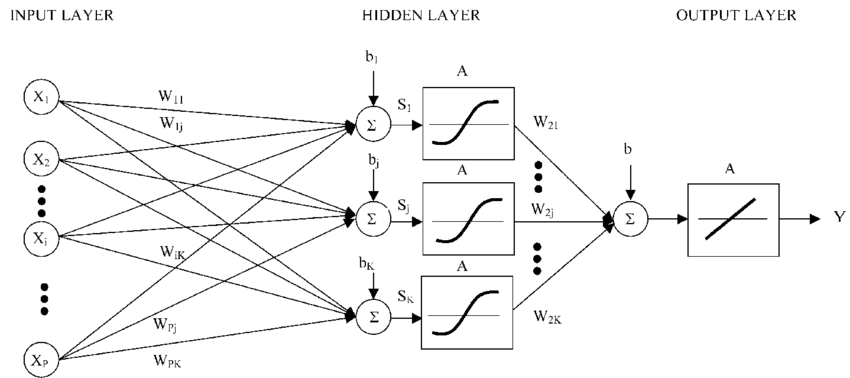
\includegraphics[width=0.9\textwidth]{ffnn.png}
        \caption{Feed Forward Neural Network (FFNN) simple visualization \cite{ffnn_structure}}
        \label{fig:enter-label}
    \end{figure}

    An FFNN consists of the following components:

    \begin{enumerate}[label={(\arabic*)}]
        \item Input Layer: The input layer receives the raw input features (denoted as $X_1, X_2, \ldots, X_p$). The number of neurons in this layer corresponds to the number of input features.
        
        \item Hidden Layers: The hidden layers transform the inputs using weighted connections and activation functions. Each neuron in a hidden layer computes a weighted sum of its inputs, adds a bias term, and applies an activation function (e.g., sigmoid, tanh, ReLU).
        
        \item Output Layer: The output layer produces the final predictions (denoted as $Y$). The number of neurons in the output layer depends on the nature of the task (e.g., a single neuron for regression, multiple neurons for classification).
    \end{enumerate}

    \paragraph{FFNN Computation}

    During a single iteration of data passing through a network, at each layer, the FFNN performs the following computations:

    \begin{enumerate}[label={(\arabic*)}]
        \item Weighted Sum: Each neuron computes a weighted sum of its inputs. For neuron $j$ in layer $l$, the weighted sum is given by:
        \[
        S_j^{(l)} = \sum_{i} W_{ij}^{(l-1)} \cdot A_i^{(l-1)} + b_j^{(l)}
        \]
        where $W_{ij}^{(l-1)}$ is the weight connecting neuron $i$ in layer $l-1$ to neuron $j$ in layer $l$, $A_i^{(l-1)}$ is the activation from the previous layer, and $b_j^{(l)}$ is the bias term.

        \item Activation Function: The weighted sum is passed through an activation function $A$ to introduce non-linearity. Common activation functions include the sigmoid function, tanh, and ReLU. For neuron $j$ in layer $l$, the activation is:
        \[
        A_j^{(l)} = A(S_j^{(l)})
        \]
        In our training we use the ReLU activation function:
        \[
        A(x) = \max(0, x)
        \]
        \item Output: In the output layer, the activations are combined to produce the final output, $Y$.
    \end{enumerate}

    \paragraph{FFNN Training}

    The FFNN is trained by minimizing a loss function, which measures the discrepancy between the predicted outputs and the actual target values. The loss function is minimized using an optimization algorithm, such as stochastic gradient descent (SGD). In this project, Mean Squared Error (MSE) loss and the Adam optimizer were used. During training, the following steps are performed iteratively:

    \begin{enumerate}[label={(\arabic*)}]
        \item Forward Propagation: Compute the activations for each layer, from the input layer to the output layer.
        
        \item Loss Calculation: Calculate the loss based on the difference between the predicted outputs and the actual target values.
        
        \item Backward Propagation: Compute the gradients of the loss with respect to the weights and biases using backpropagation.
        
        \item Weight Update: Update the weights and biases using the computed gradients to minimize the loss.
    \end{enumerate}

    This process continues until the loss converges to a minimum value or a predefined number of iterations is reached.

    The simplicity of the FFNN's architecture makes it a powerful baseline model for various tasks, including regression and classification, providing a solid foundation for comparison with more complex models. For our implementation we use the PyTorch \texttt{nn.Linear} module.

\subsubsection{\emph{Long Short Term Memory (LSTM)}}
    The LSTM Recurrent Neural Network was introduced in \cite{hochreiter1997} over 20 years ago but since has become a popular model for time series regression due to its ability to take in and learn from sequences in past data. LSTM networks are a type of recurrent neural network (RNN) designed to capture long-term dependencies and mitigate the vanishing gradient problem commonly encountered in traditional RNNs. LSTMs are particularly effective for sequence prediction tasks such as language modeling, time series forecasting, and speech recognition. Here’s a detailed explanation of how LSTMs work:

    \paragraph{LSTM Structure}
    \begin{figure}[H]
        \centering
        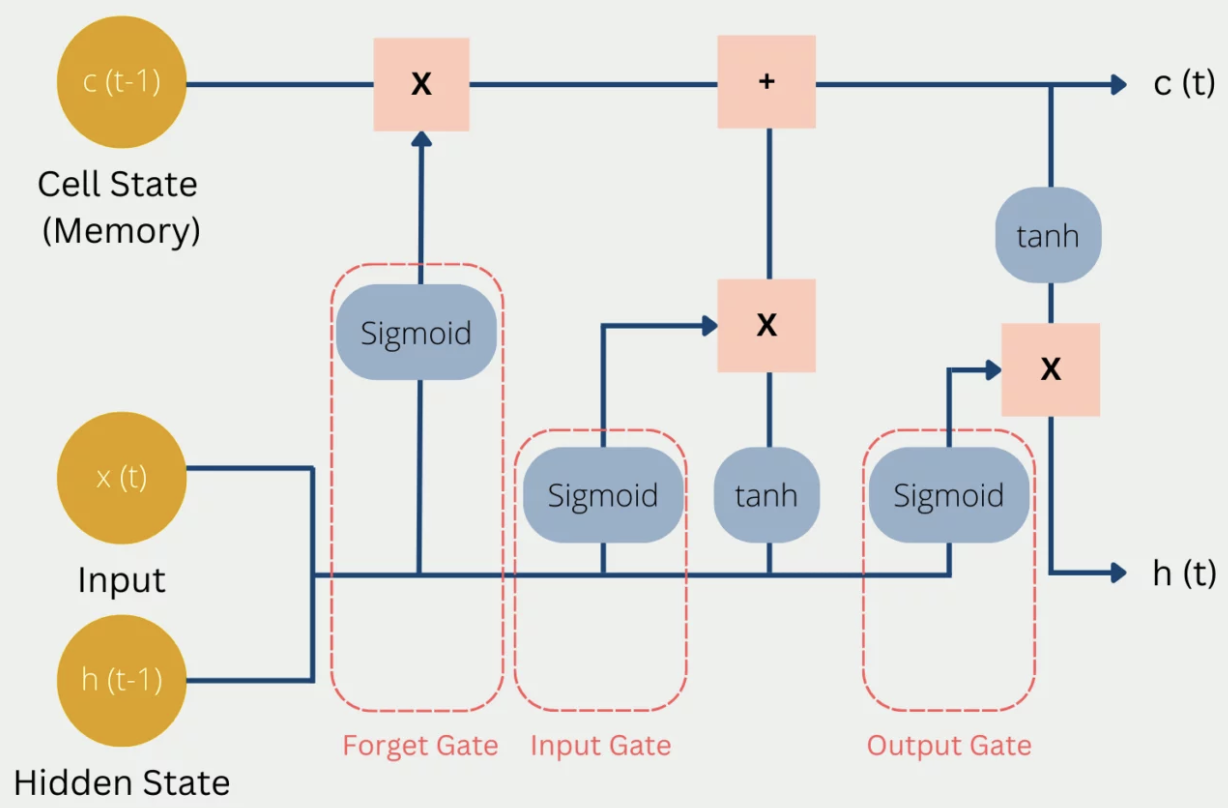
\includegraphics[width=0.7\textwidth]{lstm.png}
        \caption{Long Short Term Memory (LSTM) simple visualization of a single unit \cite{lstm_structure}.}
        \label{fig:enter-label}
    \end{figure}

    An LSTM unit consists of a cell state, hidden state, and three main gates: the input gate, forget gate, and output gate. These gates control the flow of information, enabling the network to retain or discard information over long sequences.

    \begin{enumerate}[label={(\arabic*)}]
        \item Cell State ($c_t$): The cell state is a memory component that carries information across time steps. It is the main pathway through which information flows in the LSTM, with only minor linear interactions. This design helps in retaining long-term dependencies.

        \item Hidden State ($h_t$): The hidden state is the output of the LSTM unit at each time step. It combines information from the cell state and the current input to produce the output.

        \item {Gates}:
        \begin{enumerate}
            \item Forget Gate ($f_t$): This gate determines what proportion of the previous cell state should be carried forward. It takes the hidden state from the previous time step ($h_{t-1}$) and the current input ($x_t$), and outputs a number between 0 and 1 for each number in the cell state $c_{t-1}$.
            % \[
            % f_t = \sigma(W_f \cdot [h_{t-1}, x_t] + b_f)
            % \]

            \item {Input Gate ($i_t$) and Candidate Cell State ($\tilde{c}_t$)}: The input gate decides how much of the new information (candidate cell state) should be added to the cell state. The candidate cell state ($\tilde{c}_t$) is created using the current input and the previous hidden state.
            % \[
            % i_t = \sigma(W_i \cdot [h_{t-1}, x_t] + b_i)
            % \]
            % \[
            % \tilde{c}_t = \tanh(W_c \cdot [h_{t-1}, x_t] + b_C)
            % \]

            \item {Output Gate ($o_t$)}: This gate determines the output of the current cell. It uses the current input and the previous hidden state to compute the output.
            % \[
            % o_t = \sigma(W_o \cdot [h_{t-1}, x_t] + b_o)
            % \]
        \end{enumerate}
    \end{enumerate}

    \paragraph{LSTM Computation}

    During a single iteration of data passing through a network, the LSTM performs the following computations at each unit:

    \begin{enumerate}[label={(\arabic*)}]
        \item {Forget Gate}: Decide what information to discard from the cell state.
        \[
        f_t = \sigma(W_f \cdot [h_{t-1}, x_t] + b_f)
        \]

        \item {Input Gate and Candidate Cell State}: Determine the new information to add to the cell state.
        \[
        i_t = \sigma(W_i \cdot [h_{t-1}, x_t] + b_i)
        \]
        \[
        \tilde{c}_t = \tanh(W_c \cdot [h_{t-1}, x_t] + b_c)
        \]

        \item {Update Cell State}: Update the cell state with the new information.
        \[
        c_t = f_t * c_{t-1} + i_t * \tilde{c}_t
        \]

        \item {Output Gate}: Determine the output based on the updated cell state.
        \[
        o_t = \sigma(W_o \cdot [h_{t-1}, x_t] + b_o)
        \]
        \[
        h_t = o_t * \tanh(c_t)
        \]
    \end{enumerate}

    \paragraph{LSTM Training}

    Training an LSTM involves similar steps to training an FFNN, with additional considerations for the sequential nature of the data. The primary goal is to minimize a loss function that measures the discrepancy between the predicted and actual target values. Here are the steps involved in training an LSTM:
    
    \begin{enumerate}[label={(\arabic*)}]
        \item {Forward Propagation}: At each time step, compute the activations and cell states for each LSTM unit, from the input layer through the hidden layers to the output layer. This involves calculating the forget gate, input gate, candidate cell state, cell state, output gate, and hidden state.
    
        \item {Loss Calculation}: Calculate the loss based on the difference between the predicted outputs and the actual target values. The Mean Squared Error (MSE) loss is commonly used for regression tasks, while cross-entropy loss is often used for classification tasks.
    
        \item {Backward Propagation Through Time (BPTT)}: Compute the gradients of the loss with respect to the weights and biases through backpropagation through time. This involves unrolling the LSTM network over the entire sequence and computing gradients at each time step, taking into account the dependencies between time steps.
    
        \item {Weight Update}: Update the weights and biases using an optimization algorithm, such as Adam or stochastic gradient descent (SGD). The weights are updated by applying the computed gradients to minimize the loss. This step is performed iteratively for each training batch until the loss converges to a minimum value or a predefined number of iterations is reached.
    \end{enumerate}

    LSTMs address the vanishing gradient problem by maintaining a more constant error gradient, which allows them to learn long-term dependencies more effectively than traditional RNNs. The gating mechanisms enable the network to decide what information to retain, what to update, and what to output at each time step, making LSTMs powerful for tasks involving sequential data. In our implementation we use the PyTorch \texttt{nn.LSTM} module


% \subsection{Gradient Boosting Decision Tree Regressor}
% \begin{itemize}
%     \item []
%     XGBoost is a machine learning library that supports gradient boosted decision trees. Decision trees have been shown to work well on high dimensional data due to their ability to capture trends between features and isolate for the most informative features at each split. However, decision trees have a tendency to over fit due to this same ability to capture trends in the data. Gradient boosting is when the outputs of multiple weak regressors (shallow decision trees) are combined to create a more powerful regressor. This method is powerful because it aims to create a model which reduces the high biases of each weak regressor while maintaining their low variances, thereby creating a reliable and accurate model. 
% \end{itemize}

\subsubsection{\emph{Gradient Boosting Decision Tree (GBDT) Regressor}}

    Introduced in the early 2000s \cite{boosting-paper}, the Gradient Boosting Decision Tree (GBDT) is a powerful ensemble learning technique that combines the predictions of multiple decision trees to produce a more accurate and robust model. The \texttt{xgboost} library is widely used for implementing GBDT due to its efficiency and scalability. GBDT is particularly effective for regression and classification tasks.

    \paragraph{GBDT Structure}
    \begin{figure}[H]
        \centering
        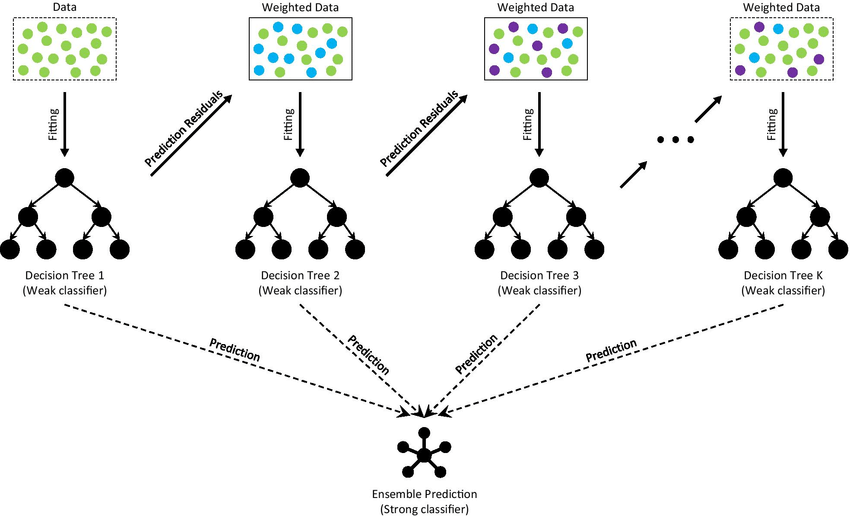
\includegraphics[width=0.9\textwidth]{gbdt.png}
        \caption{Gradient Boosting Decision Tree (GBDT) visualization \cite{gbdt_structure}}
        \label{fig:enter-label}
    \end{figure}

    A GBDT model consists of an ensemble of decision trees, where each tree is trained to correct the errors of its predecessor. The main components of GBDT include:

    \begin{enumerate}[label={(\arabic*)}]
        \item {Base Learners}: Each base learner is a decision tree, typically a shallow tree with limited depth to avoid overfitting.
        
        \item {Ensemble Method}: The ensemble method involves training multiple decision trees sequentially, where each subsequent tree is trained on the residual errors of the previous trees.
    \end{enumerate}

    \paragraph{GBDT Computation}

    The GBDT performs the following computations during training and prediction:

    \begin{enumerate}[label={(\arabic*)}]
        \item {Initialization}: The model starts with an initial prediction, usually the mean of the target values for regression tasks.
        
        \item {Training Iterations}: For each iteration $m$:
        \begin{enumerate}
            \item {Residual Calculation}: Compute the residual errors between the actual target values and the current predictions.
            \[
            r_i^{(m)} = y_i - \hat{y}_i^{(m-1)}
            \]
            where $y_i$ is the actual target value and $\hat{y}_i^{(m-1)}$ is the prediction from the previous iteration.
            
            \item {Fit Base Learner}: Train a new decision tree to predict the residuals $r_i^{(m)}$.
            
            \item {Update Predictions}: Update the predictions by adding the weighted predictions of the new tree.
            \[
            \hat{y}_i^{(m)} = \hat{y}_i^{(m-1)} + \nu f_m(x_i)
            \]
            where $\nu$ is the learning rate and $f_m(x_i)$ is the prediction from the $m$-th tree.
        \end{enumerate}
        
        \item {Final Prediction}: The final prediction is the sum of the initial prediction and the weighted predictions of all the trees.
        \[
        \hat{y}_i = \hat{y}_0 + \sum_{m=1}^{M} \nu f_m(x_i)
        \]
    \end{enumerate}

    \paragraph{GBDT Training}

    The training process for GBDT involves minimizing a loss function through an iterative process. The main steps are:

    \begin{enumerate}[label={(\arabic*)}]
        \item {Initialization}: Initialize the model with the mean of the target values.

        \item {Iterative Training}: For each iteration, compute the residuals, fit a new decision tree to the residuals, and update the model's predictions.
        
        \item {Loss Minimization}: The residuals represent the gradients of the loss function with respect to the predictions. By fitting trees to these residuals, GBDT effectively performs gradient descent in the function space.

        \item {Hyperparameter Tuning}: Optimize hyperparameters such as the number of trees, tree depth, and learning rate to improve the model's performance and prevent overfitting.
    \end{enumerate}

    Gradient Boosting Decision Trees, implemented using the \texttt{xgboost} library, offer a powerful approach to regression tasks by sequentially improving the model through the correction of residual errors. The ensemble nature of GBDT allows it to capture complex patterns and interactions in high dimensional data. This method is powerful because it aims to create a model which reduces the high biases of each weak regressor while maintaining their low variances, thereby creating a reliable and accurate model. 

\subsubsection{Benchmarks}

To evaluate the performance of our machine learning models, we compare them against well-established financial models: the Capital Asset Pricing Model (CAPM), the Fama-French 3-Factor (FF3) model, and the Fama-French 5-Factor + Momentum (FF6) model. These benchmarks provide a solid foundation for understanding the added value of our models in terms of excess returns (alpha) and risk-adjusted performance.

The CAPM is a foundational model that describes the relationship between systematic risk and expected return for assets, particularly stocks. It serves as a baseline for expected returns based on the risk-free rate, the stock's beta, and the expected market return.

The FF3 model expands on CAPM by including two additional factors: the size of companies (small vs. large) and the book-to-market value (value vs. growth). This model helps capture the variations in stock returns that cannot be explained by market risk alone.

The FF6 model further extends the FF3 model by adding three more factors: profitability, investment patterns, and momentum. This comprehensive model provides a more detailed view of the factors influencing stock returns and serves as a rigorous benchmark for evaluating the performance of advanced machine learning models.

\begin{table}[H]
    \centering
    \begin{tabular}{|c|c|c|}
        \hline
        Range (Years) & Market Type & Description \\
        \hline
        1980-1980 & 
\includegraphics[height=10pt]{green_line.png} Bullish & Market growth in early 1980. \\
        1981-1981 & 
\includegraphics[height=10pt]{red_line.png} Bearish & High inflation and interest rates. \\
        1982-1986 & 
\includegraphics[height=10pt]{green_line.png} Bullish & Post-recession recovery and growth. \\
        1987-1987 & 
\includegraphics[height=10pt]{red_line.png} Bearish & Black Monday market crash. \\
        1988-1989 & 
\includegraphics[height=10pt]{green_line.png} Bullish & Market rebound after crash. \\
        1990-1990 & 
\includegraphics[height=10pt]{red_line.png} Bearish & Recession due to Gulf War. \\
        1991-1999 & 
\includegraphics[height=10pt]{green_line.png} Bullish & Dot-com bubble driven growth. \\
        2000-2002 & 
\includegraphics[height=10pt]{red_line.png} Bearish & Dot-com bubble burst. \\
        2003-2007 & 
\includegraphics[height=10pt]{green_line.png} Bullish & Economic growth and low rates. \\
        2008-2008 & 
\includegraphics[height=10pt]{red_line.png} Bearish & Global financial crisis. \\
        2009-2017 & 
\includegraphics[height=10pt]{green_line.png} Bullish & Recovery post-2008 crisis. \\
        2018-2018 & 
\includegraphics[height=10pt]{red_line.png} Bearish & Trade war and global slowdown. \\
        2019-2019 & 
\includegraphics[height=10pt]{green_line.png} Bullish & Continued economic recovery. \\
        2020-2020 & 
\includegraphics[height=10pt]{red_line.png} Bearish & COVID-19 pandemic impact. \\
        2021-2021 & 
\includegraphics[height=10pt]{green_line.png} Bullish & Post-pandemic economic recovery. \\
        2022-2022 & 
\includegraphics[height=10pt]{red_line.png} Bearish & Inflation and interest rate concerns. \\
        2023-2023 & 
\includegraphics[height=10pt]{green_line.png} Bullish & Continued economic rebound. \\
        \hline

    \end{tabular}
    \caption{Years when the market was either bullish or bearish and a potential reason why for each.}
    \label{tab}
\end{table}

We also distinguish between different market conditions by categorizing years as either bullish (strong market returns) or bearish (weak market returns) in Table 2. This classification allows us to analyze how our models perform under varying economic conditions. For instance, we mark the year 2020 as bearish due to the COVID-19 pandemic's impact on markets, despite the eventual recovery.

By comparing our models' performance against these benchmarks, we aim to determine their ability to generate significant and consistent alpha. We perform a detailed analysis of the models' alphas and betas during bullish and bearish periods to assess their robustness and adaptability to different market environments. This comprehensive evaluation ensures that our findings are grounded in rigorous financial theory and practical market dynamics.


% \subsection{Motivation}
% We decided to utilize the Fama French Industry Portfolios due to their high diversification and accessibility through exchange-traded funds (ETFs) for each industry. These portfolios provide a practical and robust framework for trading strategies, ensuring our approach remains applicable in real-world scenarios. Moreover, the availability of comprehensive and free historical data on Kenneth French's website allows for effective model training and backtesting.

% % We decided on using the 10-industry and 49-industry value-weighted portfolios after running simple backtests on all portfolios where we trained with data from 1926-2004 and tested on data from 2004-2024. We noticed that the 10-industry models did really well in the early test data. Further, we noticed that the 49-industry did consistently well on all the test data. 

% % For all industry portfolios, the Fama French website has data for equal-weighted and value-weighted. We decided on using value-weighted because value-weighted portfolios give more weight to companies with higher market caps, which more accurately reflects the impact of larger companies on the market and aligns the portfolio more closely with market indices and real-world investment scenarios. This approach tends to reduce overall volatility and offer better risk management as larger companies are generally more stable and less susceptible to sharp declines compared to smaller, more volatile stocks. Moreover, value-weighted portfolios provide a more accurate representation of the economic footprint of industries, as larger companies contribute more significantly to economic activity.

% % Note that the 10-industry portfolios are relatively "easy" to trade since there are few industries to track. This means that we will have less transactions and thus less commission fees. Further, 49-industry portfolio is the portfolio with the most number of industries, which means that it is the most diverse. This diversity can help reduce risk and increase returns. However, because of the large number of industries (and thus ETFs) to track, there will be more transactions and thus more commission fees.

% Our strategy involves testing three distinct models, each with unique architectures and strengths, to evaluate their performance in predicting industry portfolio returns. The Feed Forward Neural Network (FFNN) serves as our baseline model due to its simplicity and proven ability to generate positive alpha in previous studies. The FFNN's straightforward architecture makes it an ideal benchmark for comparison.

% We selected the Long Short-Term Memory (LSTM) model because its architecture is designed to capture dynamic relationships within time-series data, making it particularly effective for financial data analysis. The LSTM's ability to handle sequential dependencies and long-term memory makes it a promising candidate for predicting market movements.

% Finally, we included the Gradient Boosting Decision Tree model known for its robustness and performance in handling high-dimensional data. GBDT's ensemble learning approach, which combines the outputs of multiple weak regressors, aims to balance bias and variance, potentially offering reliable and accurate predictions.

% By comparing these models against traditional benchmarks such as the CAPM, Fama-French 3-factor, and Fama-French 6-factor models, we aim to assess their ability to outperform standard approaches and provide excess returns (alpha) that are not explained by conventional market factors. Additionally, we investigate the performance of our models across different market regimes, identifying periods of bullish and bearish trends to understand their effectiveness under varying market conditions. Lastly, we explore the impact of past data lags on model performance, evaluating the predictive power of different time horizons in forecasting industry portfolio returns.

% Through this comprehensive analysis, we seek to identify robust and adaptable machine learning models capable of enhancing trading strategies and delivering superior returns in the context of Fama French Industry Portfolios.

\subsection{Motivation}

In this study, we aim to explore the potential of machine learning models in improving trading strategies based on the Fama French Industry Portfolios, leveraging their diverse and comprehensive data to develop robust, adaptable, and high-performing investment models. The motivation for this study stems from the desire to enhance trading strategies through the application of advanced machine learning techniques. The Fama French Industry Portfolios provide a robust framework for developing diversified investment strategies, given their comprehensive coverage of various industries and the availability of extensive historical data. These portfolios are not only well-documented but also accessible through exchange-traded funds (ETFs), making them practical for real-world trading applications.

Our decision to utilize the Fama French Industry Portfolios is based on their ability to represent a diverse set of market sectors, which allows for a broad interaction between industry-specific trends and behaviors. This diversity is crucial for creating a well-rounded strategy that can potentially mitigate risks and capitalize on opportunities across different market segments. By leveraging the rich historical data available on Kenneth French's website, we can effectively train and backtest our models, ensuring their reliability and robustness.

For all industry portfolios, the Fama French website has data for equal-weighted and value-weighted. We decided on using value-weighted because value-weighted portfolios give more weight to companies with higher market caps, which more accurately reflects the impact of larger companies on the market and aligns the portfolio more closely with market indices and real-world investment scenarios. This approach tends to reduce overall volatility and offer better risk management as larger companies are generally more stable and less susceptible to sharp declines compared to smaller, more volatile stocks. Moreover, value-weighted portfolios provide a more accurate representation of the economic footprint of industries, as larger companies contribute more significantly to economic activity. Data for equal-weighted portfolio model performance is in appendix.

We chose to focus on three machine learning models—FFNN, LSTM networks, and GBDT regressors—each bringing unique strengths to the table. The FFNN serves as a baseline due to its simplicity and proven effectiveness in financial applications. The LSTM model is selected for its ability to capture temporal dependencies in sequential data, which is particularly relevant for financial time series. The GBDT model is included for its robustness and capability to handle high-dimensional data, often outperforming simpler models in various regression tasks.

Our approach includes a thorough comparison of these models against traditional financial benchmarks like the CAPM, FF3, and FF6 models. We also assess the performance of our models across different market regimes—bullish and bearish—to understand their effectiveness under varying economic conditions. By doing so, we aim to identify machine learning models that not only generate consistent alpha but also adapt well to different market environments, thereby providing a reliable tool for enhancing trading strategies.

\medskip

\section{Related Work}

The prediction of next-day stock price movements has been a significant area of research within the field of financial machine learning. One of the pioneering works in this domain is by Fischer and Krauss (2018), who demonstrated the superiority of Long Short-Term Memory (LSTM) networks over traditional feedforward neural networks (FFNN) for predicting next-day stock movements. Their study showed that LSTMs could effectively capture temporal dependencies in financial time series data, leading to improved prediction accuracy compared to FFNNs \cite{fischer2018}. Another notable study by Weng, Ahmed, and Megahed (2017) explored the application of Gradient Boosting Decision Trees (GBDT) for next-day stock movement prediction. They found that GBDTs outperformed FFNNs by leveraging the model's ability to handle high-dimensional data and capture complex non-linear relationships between features. This study highlighted the potential of ensemble learning techniques in financial prediction tasks \cite{weng2017}. Furthermore, Eachempati et al. (2019) utilized LSTM networks for financial sentiment analysis, demonstrating how integrating sentiment data from news and social media can enhance the prediction of stock price movements. Their work underscored the importance of incorporating diverse data sources to improve the robustness and accuracy of predictive models in finance \cite{eachempati}.

The development of industry trading strategies has also garnered considerable attention in financial research. A seminal work by Fama and French (1997) introduced the Fama French Industry Portfolios, which have become a standard framework for analyzing industry-specific returns. Their methodology involves constructing portfolios based on industry classifications and has been widely adopted in both academic research and practical trading strategies \cite{french1997}. Recent studies have leveraged machine learning models to enhance industry trading strategies. For instance, Nevasalmi et al. (2020) applied GBDTs to forecast daily returns of the S\&P 500 and demonstrated the model's ability to outperform traditional linear models. Their approach involved using a comprehensive set of features, including technical indicators and macroeconomic variables, to capture industry-specific trends and generate more accurate predictions \cite{nevasalmi2020forecasting}. Additionally, the work by Tsantekidis et al. (2017) on using deep learning models for financial prediction emphasized the effectiveness of LSTM networks in capturing the sequential nature of financial data. They applied their models to various industry sectors and showed that deep learning models could significantly enhance the performance of industry-specific trading strategies compared to conventional approaches \cite{tsantekidis2017}. Overall, the integration of advanced machine learning techniques in industry trading strategies has demonstrated substantial potential in generating superior returns. These studies highlight the importance of using diverse and comprehensive datasets, as well as sophisticated model architectures, to capture the intricate dynamics of financial markets and improve the efficacy of trading strategies.

% \section{Methods}
% We performed a rolling window training and testing strategy where we trained our model from the start of the data (1926) to the current year (excluding) and then tested out its predictions on current year up until the next year (excluding). We then moved the window forward by one year and repeated the process. This allowed us to see how well our model performed in a real-world scenario where we are constantly updating our model with new data.

% For finding the best data and model configurations we tested all permutations of the following parameters:
% \begin{enumerate}[label={(\arabic*)}]
%     \item \textbf{Number of Industries}: 5, 10, 12, 17, 30, 48, 49
%     \item \textbf{Model Architecture}: FFNN, LSTM, GBDT
%     \item \textbf{Day Lag}: 5, 22
%     \item \textbf{Portfolio Strategy Type}: Max-Min Long-Short, Weighted Long-Short, Max Long
%     \item \textbf{Industry Data Weighing}: Value, Equal
% \end{enumerate}

% \subsection{Data Processing}
% We took in the Fama French Industry Portfolios data and preprocess it to be used in our models. We first clean the data by removing any missing values (marked -99.99 in the data) and normalize the valid data (non-missing values). Each model inputs the past $5$ (week) or $22$ (month) days of data to predict the returns of the next day. We then split the data into training and validation sets where the training set is from 1926 to the year we are testing (exclusive) on and the validation set is the year we are testing on. This validation set has no influence on the training of the model and is only used to see if the model is learning between epochs. 

% \subsection{Training}
% \subsubsection{FFNN}
% The model had 4 linear layers: input, 2 hidden, output. The input layer had as many neurons as the number of industries in the Fama French Industry Portfolios times the number of days of lag data we are inputting. It had 2 hidden layers with 32 and 16 neurons, respectively. The output layer had as many neurons as the number of industries. The loss function was MSE loss, the activation function was ReLU, and the optimizer was Adam with a learning rate of 0.001. There was a dropout of 0.1 after year linear layer and the model was trained for 5 epochs. We train with a batch size of 32.

% \subsubsection{LSTM}
% The model had 2 layers: 1-layer LSTM, linear output layer. The 1-layer LSTM had 50 hidden units. The output from this LSTM layer got fed into a ReLU activation function, then a linear layer with an input size equal to the number of hidden units and output size equal to the number of industries (10 or 49). The loss function was MSE loss, the optimizer was Adam with a learning rate of 0.001, and the model was trained for 5 epochs. We train with a batch size of 32.

% \subsubsection{GBDT}
% The model was an \texttt{xgboost} XGBRegressor model with an objective set to \texttt{reg:squarederror}, signifying it is for a regression task and to be trained with squared error loss. We train with a batch size of 32.

% \subsection{Backtesting}
% We did a rolling backtest. Our first model was trained with data from 1926 to 1979 and used for predictions of data in 1980. We then retrained the model with data from 1926 to 1980 and used it for predictions of data in 1981. We repeated this process until we reached 2020. In the appendix, we have plots and tables for data up to 2024 (exclusive). We decided not to include the past 4 years in our analysis due to the unique nature of the market during and post pandemic. Once a model (for an individual year) is trained, for each day in the validation year, given the past $n$ days of data, we predict the returns of each industry for the next day. We then apply one of our portfolio creation strategies. We tested the following strategies:
% \begin{enumerate}[label={(\arabic*)}]
%     \item \textbf{Max-Min Long-Short (LS)}: Invest in the top decile of industries which our model predicts to have the highest returns and short the bottom decile of industries which our model predicts to have the lowest returns. We weight the long and short positions according to the predicted returns such that the sum of the weights is 0.
%     \item \textbf{Weighted Long-Short (LS)}: Invest in all industries according to the model prediction of their returns. We long the industries that are predicted to have positive returns and short the industries that are predicted to have negative returns. We weight the long and short positions according to the predicted returns such that the sum of the weights is 0.
%     \item \textbf{Max Long (L)}: Go long in the industry which our model predicts to have the highest return.
% \end{enumerate}

% After all of the years were predicted, we ran benchmarks to calculate alphas, betas, and Sharpe ratio.

% We then perform a linear regression of our model's portfolio returns to the FF6 benchmark returns and calculate the alpha (checking its significance) and beta of our models to see if they are able to outperform FF6 and to what extent they are described by it. For a particular set of number of industries, portfolio creation strategy, and input day lags, we plot the cumulative returns of all three models (LSTM, FFNN, XGBoost) and compare it to the market's return over the same time period. We also note the alpha and beta of each model during bearish and bullish markets to see if our models perform particularly well in one regime or the other. To do this we concatenate the returns of all the years in the same market regime and perform a linear regression on the returns of our models to the FF6 benchmark returns.

\section{Methods}

Our methodology involves a systematic rolling window training and testing strategy to rigorously evaluate the performance of our machine learning models. We start by training each model on historical data from 1926 up to, but not including, the current year. The trained model is then tested on data from the current year up to, but not including, the next year. This process is repeated annually, progressively moving the training window forward by one year. This approach mimics real-world conditions where models are continually updated with new data, ensuring their relevance and adaptability over time.

To identify the optimal data and model configurations, we exhaustively test all permutations of the following parameters:

\begin{enumerate}[label={(\arabic*)}]
    \item {Number of Industries}: 5, 10, 12, 17, 30, 48, 49
    \item {Model Architecture}: FFNN, LSTM, GBDT
    \item {Day Lag}: 5, 22
    \item {Portfolio Strategy Type}: Max-Min Long-Short, Weighted Long-Short, Max Long
    \item {Industry Data Weighting}: Value, Equal
\end{enumerate}

\subsection{Data Processing}
We preprocess the Fama French Industry Portfolios data to ensure it is suitable for input into our models. Initially, we clean the data by removing any missing values (marked as -99.99 in the dataset) and normalize the valid data points. Each model is provided with the past $5$ (week) or $22$ (month) days of data to predict the returns of the next day. The dataset is then split into training and testing sets, where the training set spans from 1926 to the year before the testing year. The testing set, comprising the current year, is used solely for evaluating model performance during training epochs without influencing the training process.

\subsection{Training}

\subsubsection{\emph{FFNN}}
The FFNN model comprises four linear layers: an input layer, two hidden layers, and an output layer. The input layer has neurons corresponding to the number of industries multiplied by the number of days of lag data. The hidden layers contain 32 and 16 neurons, respectively, while the output layer has neurons corresponding to the number of industries. The model uses Mean Squared Error (MSE) loss, ReLU activation functions, and the Adam optimizer with a learning rate of 0.001. A dropout rate of 0.1 is applied after each linear layer, and the model is trained for 5 epochs.

\subsubsection{\emph{LSTM}}
The LSTM model consists of a single LSTM layer with 50 hidden units and a subsequent linear output layer. The LSTM layer processes the sequential data, feeding its output through a ReLU activation function before reaching the final linear layer. The model uses MSE loss and the Adam optimizer with a learning rate of 0.001. Training is conducted over 5 epochs.

\subsubsection{\emph{GBDT}}
The GBDT model employs the \texttt{xgboost} library's XGBRegressor, configured for regression tasks using squared error loss. The objective function is set to \texttt{reg:squarederror}, reflecting its focus on minimizing the squared error during training.

\subsection{Backtesting}
Our backtesting evaluates the performance of our models over an extended historical period. We implement a rolling window approach, where models are continuously updated and tested on new data each year, mimicking real-world conditions. Initially, the models are trained on data from 1926 to 1979 and tested on data from 1980. Subsequently, the models are retrained with data extended to include 1980 and tested on data from 1981. This iterative process continues up to 2020, with additional plots and tables provided for data up to 2024 in the appendix. This exclusion accounts for the unique market conditions during and post the COVID-19 pandemic; we will note though that our strategy performs just as well post pandemic.

For each testing year, daily predictions are made using the past $n$ days of data. These predictions inform the creation of portfolios based on one of three strategies:
\begin{enumerate}[label={(\arabic*)}]
    \item {Max-Min Long-Short}: Long the top decile of industries with the highest predicted returns and short the bottom decile with the lowest predicted returns, with weights adjusted so the sum of the weights is zero.
    \item {Weighted Long-Short}: Long industries predicted to have positive returns and short those predicted to have negative returns, with weights proportional to the predicted returns and adjusted to sum to zero.
    \item {Max Long}: Long the single industry predicted to have the highest return.
\end{enumerate}

% After generating predictions for all testing years, we benchmark our models by calculating alphas, betas, and Sharpe ratios. Linear regression is used to compare model portfolio returns to the FF6 benchmark returns, determining the significance of the alpha and the extent to which our models are explained by the benchmark. This thorough evaluation helps to understand the robustness and performance of our models across different market conditions.

After generating predictions for all testing years, we benchmark our models by calculating alphas, betas, and Sharpe ratios. Linear regression is used to compare model portfolio returns to the FF6 benchmark returns, determining the significance of the alpha and the extent to which our models are explained by the benchmark. To gain deeper insights, we also analyze the performance of our models across different market conditions, categorizing years as bullish or bearish. This allows us to evaluate how our models perform in varying economic environments.

Furthermore, we assess model performance over different time periods: 1980-1995, 1996-2010, and 2011-2020. This segmented analysis helps us understand how the models adapt to changing market dynamics over decades. By comparing alphas, betas, and Sharpe ratios across these periods, we can identify trends and evaluate the consistency of model performance. This comprehensive evaluation ensures a thorough understanding of the robustness and effectiveness of our models across multiple dimensions and market conditions.

\medskip

\section{Results}
% Our best model configuration was using the LSTM model trained on the value-weighted Fama French 49 Industry Portfolio Returns using a 5-day lag and calculating our strategy returns using the Max-Min Long-Short strategy. We compared the best model to other models by comparing to other models by deviating by one parameter and showing plots of cumulative returns, bar graphs of yearly raw returns, and benchmark analysis tables.

% We show our best model's returns in blue and the market's returns in black. The green and red  regions on the plots represent times of bullish and bearish market movements, respectively. The accompanying bar graphs on Figure \ref{fig:timeperiods}, \ref{fig:model_comp}, \ref{fig:seq_len_comp}, \ref{fig:data_weighing_comp}, show the raw strategy returns and market returns for each month during the testing period. For the tables, we denote significant alphas with a * next to their corresponding value and compute all values except for in Table \ref{tab:benchmarks} during the periods from 1980 to 1995, 1995 to 2010, and 2010 to 2020, respectively.

Our highest alpha producing strategy had configuration that utilized the LSTM model trained on the value-weighted Fama French 49 Industry Portfolio Returns using a 5-day lag, with returns calculated using the Max-Min Long-Short strategy. Let this configuration be labeled as $H$. To evaluate the performance of our optimal strategy, we compared it to other configurations by varying one parameter at a time and analyzing the results. We provide visualizations of cumulative returns, bar graphs depicting yearly raw returns, and tables summarizing benchmark analysis.

We show our best strategy's returns in blue and the market's returns in black. The green and red regions on the plots represent times of bullish and bearish market movements, respectively. The accompanying bar graphs in Figures \ref{fig:timeperiods}, \ref{fig:model_comp}, \ref{fig:seq_len_comp}, and \ref{fig:data_weighing_comp} illustrate the raw strategy returns and market returns for each month during the testing period. In the tables, we denote significant alphas with an asterisk (*) next to their corresponding value and compute all values, except for those in Table \ref{tab:benchmarks}, during the periods from 1980 to 1995, 1995 to 2010, and 2010 to 2020, respectively.


\newpage

% \newgeometry{left=0cm,right=0cm,bottom=0cm}
\begin{figure}[H]
    \centering
    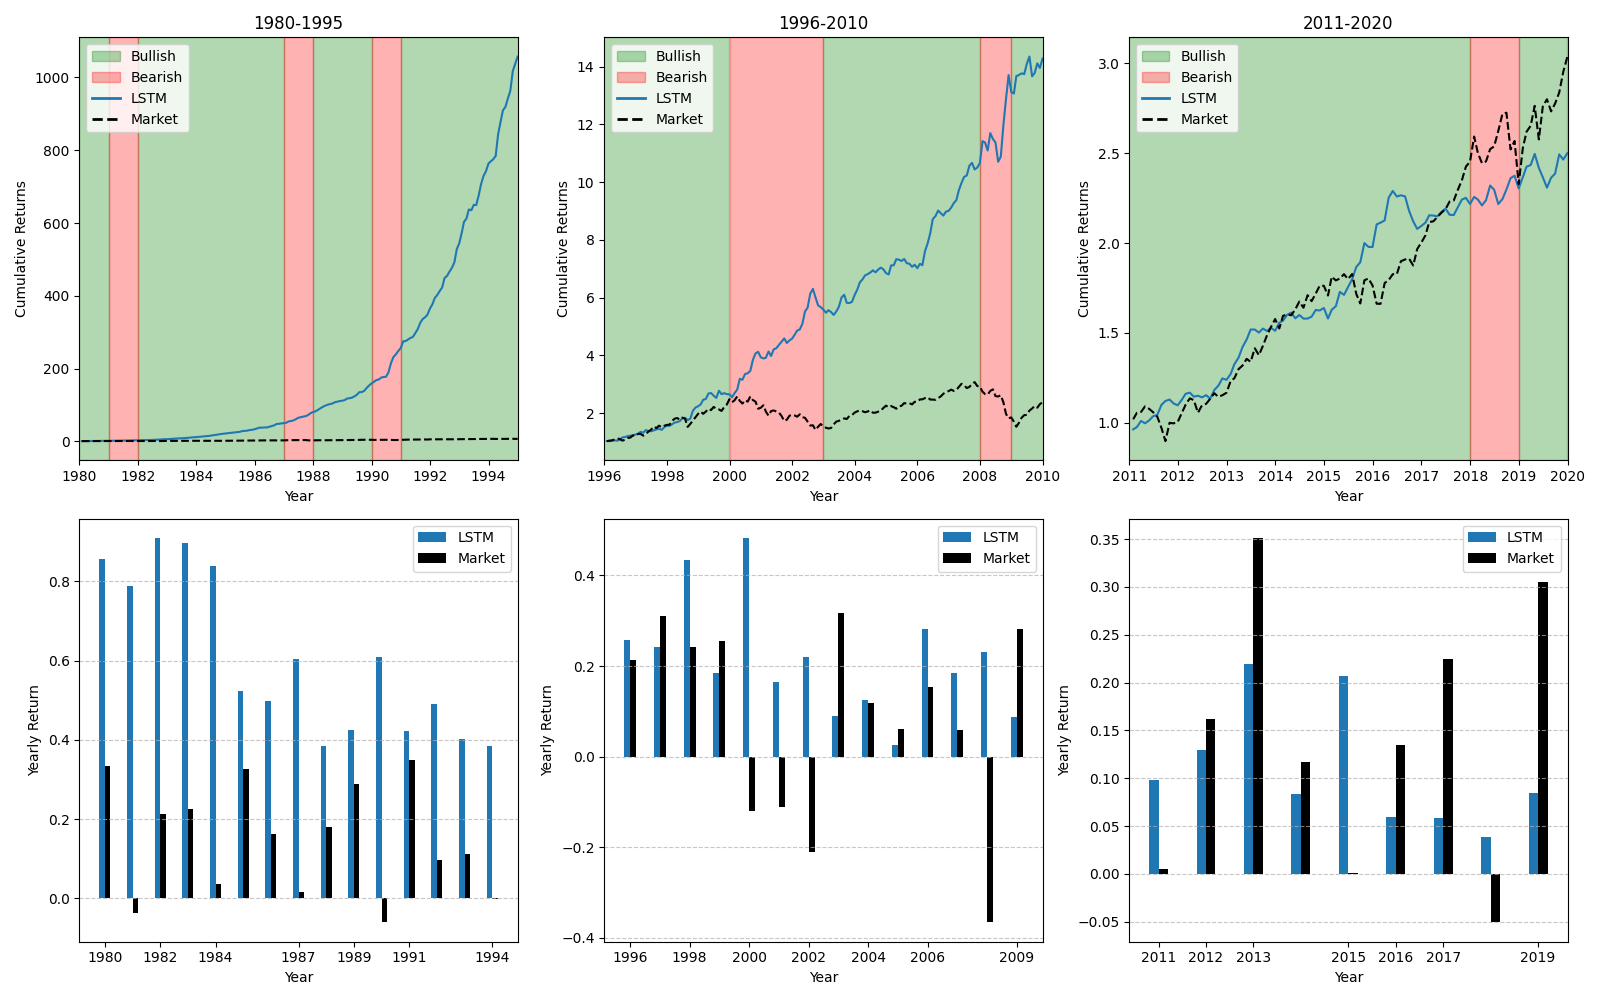
\includegraphics[width=0.8\textwidth]{2020_plot2_model_comparison_timeperiods.png}
    \caption{Monthly cumulative returns and annualized raw returns of best strategy in three separate time periods.}
    \vspace{-10pt}
    \label{fig:timeperiods}
\end{figure}


\begin{table}[h]
    \centering
    \begin{minipage}{0.4\textwidth}
        \centering
        % 2020 table
        \begin{tabular}{lcccc}
            \toprule
            & $\alpha$ (Annual) & $\beta$ & Sharpe Ratio \\
            \midrule
            CAPM & 0.10* (28.54) & 0 & 0.67 \\
            FF3  & 0.10* (28.36) & 0.01 & 0.67 \\
            FF6  & 0.09* (27.69) & 0.02 & 0.67 \\
            \bottomrule
        \end{tabular}
        % 2024 table
        % \begin{tabular}{lcccc}
        %     \toprule
        %     & $\alpha$ (Annual) & $\beta$ & Sharpe Ratio \\
        %     \midrule
        %     CAPM & 0.09* (28.18) & 0.01 & 0.65 \\
        %     FF3  & 0.09* (27.00) & 0.01 & 0.65 \\
        %     FF6  & 0.09* (27.47) & 0.02 & 0.65 \\
        %     \bottomrule
        % \end{tabular}
        \caption{Best strategy CAPM, FF3, and FF6 benchmarks. $\alpha$ is daily and in percent. * signifies significant $\alpha$.}
        \label{tab:benchmarks}
    \end{minipage}
    \hspace{0.05\textwidth} % Adjust space between tables
    \begin{minipage}{0.4\textwidth}
        \centering
        % 2020 table
        \begin{tabular}{lcccc}
            \toprule
             & Period & $\alpha$ (Annual) & $\beta$ & Sharpe Ratio \\
            \midrule
            \multirow{3}{*}{Total} & 1980-1995 & 0.16* (51.57) & 0.01 & 1.49 \\
                                   & 1995-2010 & 0.06* (17.43) & 0.03 & 0.40 \\
                                   & 2010-2020 & 0.04* (10.65) & 0.04 & 0.38 \\
            \midrule
            \multirow{3}{*}{Bullish} & 1980-1995 & 0.15* (50.32) & -0.00 & 1.05 \\
                                     & 1995-2010 & 0.05* (15.36) & 0.03 & 0.33 \\
                                     & 2010-2020 & 0.04* (11.49) & 0.04 & 0.38 \\
            \midrule
            \multirow{3}{*}{Bearish} & 1980-1995 & 0.17* (58.50) & 0 & 0.45 \\
                                     & 1995-2010 & 0.07* (21.03) & 0.02 & 0.26 \\
                                     & 2010-2019 & 0.02 (4.35) & 0.05 & 0.09 \\
            \bottomrule
        \end{tabular}
        \caption{Best strategy FF6 benchmarks for bullish and bearish markets as well as for different time periods. * signifies significant $\alpha$.}
        \label{tab:regimes}
        % 2024 table
        % \begin{tabular}{lcccc}
        %     \toprule
        %      & Period & $\alpha$ (Annual) & $\beta$ & Sharpe Ratio \\
        %     \midrule
        %     \multirow{3}{*}{Total} & 1980-1995 & 0.16* (51.57) & 0.01 & 1.49 \\
        %                            & 1995-2010 & 0.06* (17.43) & 0.03 & 0.40 \\
        %                            & 2010-2024 & 0.05* (14.69) & 0.03 & 0.41 \\
        %     \midrule
        %     \multirow{3}{*}{Bullish} & 1980-1995 & 0.15* (50.32) & -0.00 & 1.05 \\
        %                              & 1995-2010 & 0.05* (15.36) & 0.03 & 0.33 \\
        %                              & 2010-2024 & 0.04* (12.37) & 0.04 & 0.38 \\
        %     \midrule
        %     \multirow{3}{*}{Bearish} & 1980-1995 & 0.17* (58.5) & 0 & 0.45 \\
        %                              & 1995-2010 & 0.07* (21.03) & 0.02 & 0.26 \\
        %                              & 2010-2014 & 0.07* (21.07) & 0.03 & 0.29 \\
        %     \bottomrule
        % \end{tabular}
    \end{minipage}
\end{table}

The strategy performs exceptionally well in the first time period (1980-1995), consistently outperforming the market with raw returns. During this period, it achieves a significant annual alpha of over 50\% across all market conditions, with the highest overall Sharpe ratio of 1.49. This indicates a very favorable risk-adjusted return compared to the market. In the second period (1995-2010), the strategy continues to generate significant alpha, though at a reduced level of around 17\% annually. Despite this reduction, the Sharpe ratio remains reasonably high at 0.40, indicating a decrease in performance potentially due to more use of similar strategies for trading. In the third period (2010-2020), while the strategy's annual alpha remains significant, it is the lowest among all time periods at approximately 10\%, with a Sharpe of ratio of 0.38. This suggests that while the strategy continues to add value, its effectiveness has diminished over time.

Notably, the market beta is consistently near zero across all time periods, benchmarks, and market conditions. This implies that the strategy's returns are largely independent of market movements. Additionally, there is minimal discrepancy in alpha values across the CAPM, FF3, and FF6 benchmarks, suggesting that the factors included in these models do not significantly explain the strategy's alpha.

% \restoregeometry

\begin{figure}[H]
    \centering
    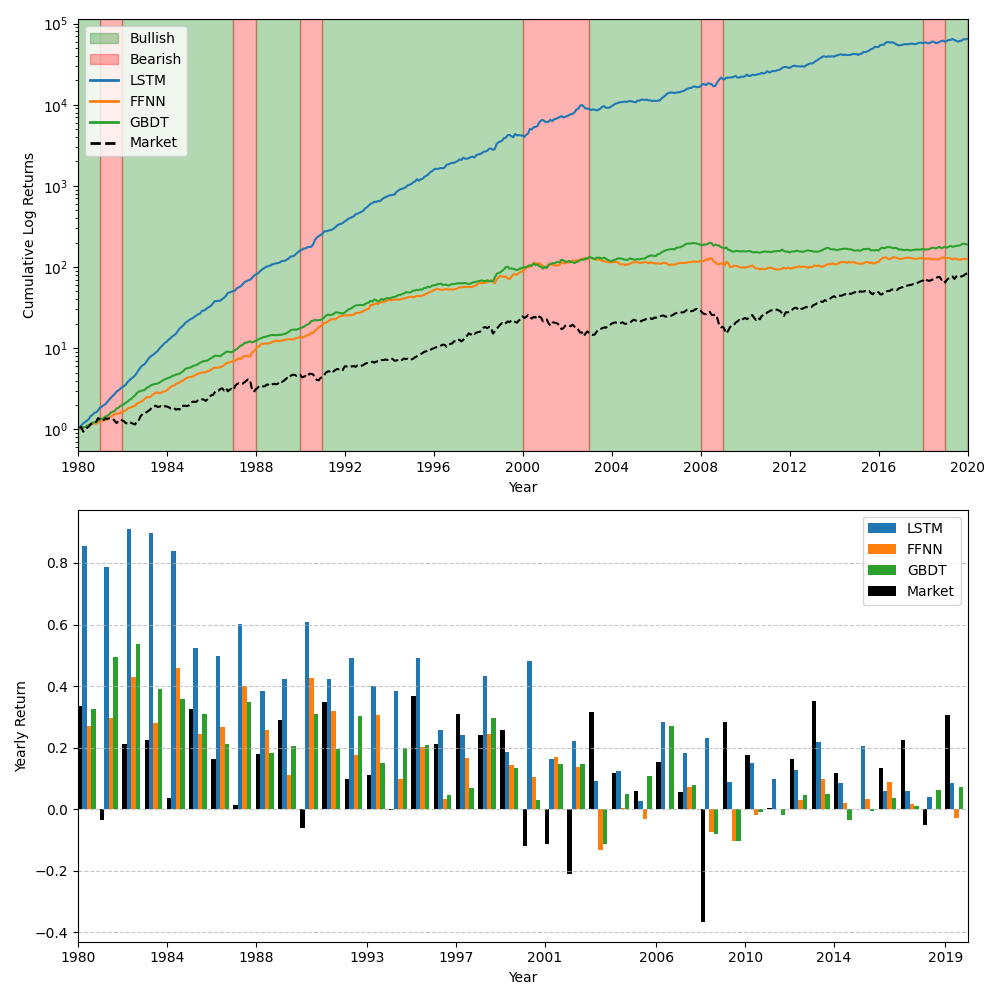
\includegraphics[width=0.9\textwidth]{2020_plot1_model_comparison.png}
    \caption{Monthly cumulative returns and raw annual returns for varying model types.}
    \label{fig:model_comp}
\end{figure}

% 2020 table
\begin{table}[H]
    \centering
    \begin{tabular}{lcccccc}
        \toprule
         & Period & $\alpha$ (Annual) & $\beta$ & Sharpe Ratio \\
        \midrule
        \multirow{3}{*}{LSTM} & 1980-1995 & 0.16* (51.57) & 0.01 & 1.49 \\
                              & 1995-2010 & 0.06* (17.43) & 0.03 & 0.40 \\
                              & 2010-2020 & 0.04* (10.65) & 0.04 & 0.38 \\
        \midrule
        \multirow{3}{*}{FFNN} & 1980-1995 & 0.07* (20.70) & -0.04 & 0.70 \\
                              & 1995-2010 & 0.01 (1.60) & 0.01 & 0.05 \\
                              & 2010-2020 & 0.01* (3.35) & -0.04 & 0.10 \\
        \midrule
        \multirow{3}{*}{GBDT} & 1980-1995 & 0.07* (21.38) & 0.05 & 0.80 \\
                              & 1995-2010 & 0.02* (4.49) & 0.01 & 0.12 \\
                              & 2010-2020 & 0.01* (1.66) & 0.02 & 0.09 \\
        \bottomrule
    \end{tabular}
    \caption{FF6 benchmark for varying model types. * signifies significant $\alpha$.}
    \label{tab:model_comp}
\end{table}

The comparison of different model architectures, as depicted in Figure 5, highlights the performance variations between LSTM, FFNN, and GBDT models over several decades. The LSTM model consistently outperforms the other architectures, especially in the earlier period (1980-1995). In the subsequent periods (1995-2010 and 2010-2020), while the LSTM's performance diminishes slightly, it still performs better than the other two model types. This consistent performance across different time periods underscores the robustness and adaptability of the LSTM model in financial market predictions, indicating the LSTM's superior ability to capture complex temporal patterns and generate high risk-adjusted returns.

In comparison, the FFNN and GBDT models exhibit more variable performance. The FFNN model shows a significant annual alpha of 20.70\% with a Sharpe ratio of 0.70 in the first period, but its effectiveness decreases considerably in later periods, with only marginally positive alphas and lower Sharpe ratios. Similarly, the GBDT model achieves a 21.38\% annual alpha and a Sharpe ratio of 0.80 in the first period, but its performance also wanes over time, with much lower alphas in the subsequent periods. These results suggest that while FFNN and GBDT models can provide some benefits in specific conditions, they lack the consistent performance and robustness demonstrated by the LSTM model.

% Overall, the data emphasizes the superiority of the LSTM model for financial market predictions due to its ability to adapt and maintain high performance across different market regimes. The consistent alpha generation and favorable Sharpe ratios of the LSTM model highlight its effectiveness in capturing market trends and providing reliable risk-adjusted returns. In contrast, the more variable performance of the FFNN and GBDT models suggests that they may be less suited for long-term, dynamic market conditions, reinforcing the preference for LSTM in developing advanced trading strategies

% 2024 table
% \begin{table}[h]
%     \centering
%     \begin{tabular}{lcccccc}
%         \toprule
%         Model Type & Period & $\alpha$ (Annual) & $\beta$ & Sharpe Ratio \\
%         \midrule
%         \multirow{3}{*}{LSTM} & 1980-1995 & 0.16* (51.57) & 0.01 & 1.49 \\
%                               & 1995-2010 & 0.06* (17.43) & 0.03 & 0.40 \\
%                               & 2010-2024 & 0.05* (14.69) & 0.03 & 0.41 \\
%         \midrule
%         \multirow{3}{*}{FFNN} & 1980-1995 & 0.07* (20.70) & -0.04 & 0.70 \\
%                               & 1995-2010 & 0.01 (1.60) & 0.01 & 0.05 \\
%                               & 2010-2024 & 0.01* (3.31) & -0.08 & 0.08 \\
%         \midrule
%         \multirow{3}{*}{GBDT} & 1980-1995 & 0.07* (21.38) & 0.05 & 0.80 \\
%                               & 1995-2010 & 0.02* (4.49) & 0.01 & 0.12 \\
%                               & 2010-2024 & 0.01* (3.23) & 0.03 & 0.14 \\
%         \bottomrule
%     \end{tabular}
%     \caption{Model Architecture Comparison}
%     \label{tab:model_comp}
% \end{table}

% 2020 table
\begin{table}[H]
    \centering
    \begin{tabular}{lcccccc}
        \toprule
        & Period & $\alpha$ & $\alpha$ (Annual) & $\beta$ & Sharpe Ratio \\
        \midrule
        \multirow{3}{*}{49 Industries} & 1980-1995 & 0.16* & 51.57 & 0.01 & 1.49 \\
                                       & 1995-2010 & 0.06* & 17.43 & 0.03 & 0.40 \\
                                       & 2010-2020 & 0.04* & 10.65 & 0.04 & 0.38 \\
        \midrule
        \multirow{3}{*}{48 Industries} & 1980-1995 & 0.16* & 53.09 & 0.02 & 1.37 \\
                                       & 1995-2010 & 0.08* & 23.28 & 0.02 & 0.48 \\
                                       & 2010-2020 & 0.02* & 5.53 & 0.03 & 0.20 \\
        \midrule
        \multirow{3}{*}{30 Industries} & 1980-1995 & 0.12* & 39.05 & 0.02 & 1.17 \\
                                       & 1995-2010 & 0.04* & 10.07 & -0.02 & 0.21 \\
                                       & 2010-2020 & 0.01* & 2.59 & -0.02 & 0.06 \\
        \midrule
        \multirow{3}{*}{17 Industries} & 1980-1995 & 0.18* & 58.77 & -0.03 & 1.29 \\
                                       & 1995-2010 & 0.08* & 21.97 & -0.03 & 0.40 \\
                                       & 2010-2020 & 0.01* & 3.68 & -0.00 & 0.09 \\
        \midrule
        \multirow{3}{*}{12 Industries} & 1980-1995 & 0.19* & 63.97 & -0.05 & 1.43 \\
                                       & 1995-2010 & 0.03* & 8.76 & -0.01 & 0.19 \\
                                       & 2010-2020 & -0.00 & -1.03 & -0.02 & -0.04 \\
        \midrule
        \multirow{3}{*}{10 Industries} & 1980-1995 & 0.24* & 88.93 & -0.06 & 1.36 \\
                                       & 1995-2010 & -0.00 & -0.39 & -0.05 & 0.01 \\
                                       & 2010-2020 & 0.01 & 1.63 & -0.01 & 0.04 \\
        \midrule
        \multirow{3}{*}{5 Industries}  & 1980-1995 & 0.1* & 29.82 & -0.05 & 0.75 \\
                                       & 1995-2010 & 0.00 & 1.3 & 0.01 & 0.03 \\
                                       & 2010-2020 & 0.00 & 1.14 & -0.02 & 0.03 \\
        \bottomrule
    \end{tabular}
    \caption{FF6 benchmark for varying number of industries in different time periods. * signifies significant $\alpha$.}
    \label{tab:number_of_industries_comparison}
\end{table}

\begin{figure}[H]
    \centering
    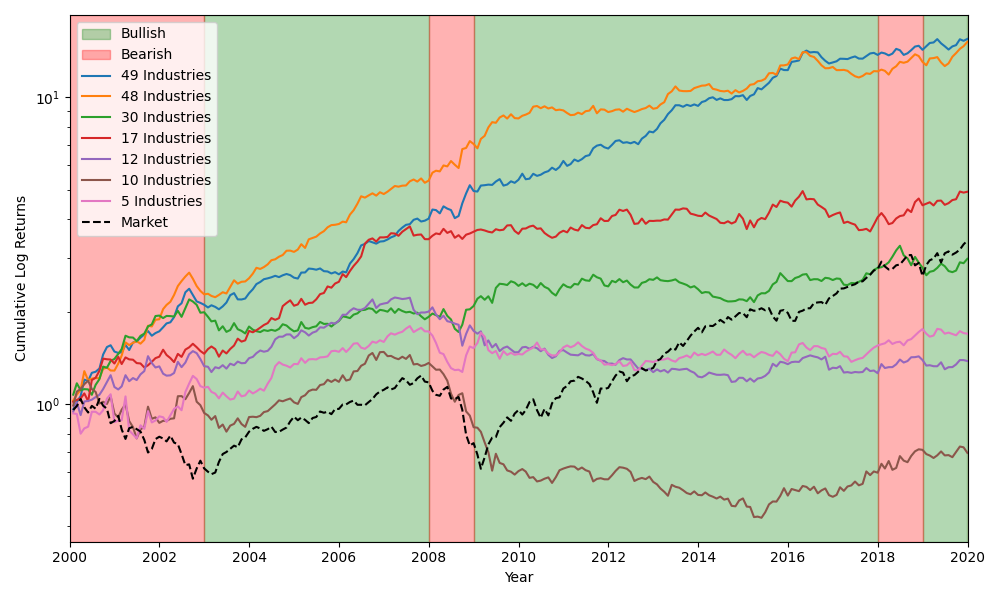
\includegraphics[width=0.7\textwidth]{2020_plot3_num_industries_comparison.png}
    \caption{Monthly cumulative returns for varying number of industries.}
    \label{fig:industry_comp}
\end{figure}

Across different periods, models trained with a higher number of industries, specifically the 49-industry and 48-industry configurations, demonstrated robust performance with significant alpha and strong Sharpe ratios. This suggests that incorporating a broad range of industries allows the model to capture diverse market dynamics, thereby enhancing its ability to generate returns and manage risk. These configurations consistently yielded high returns, especially in earlier periods (1980-1995), where market inefficiencies could have been more prevalent, allowing well-diversified models to capitalize on a wider array of opportunities.

On the other hand, configurations with fewer industries, such as the 5-industry and 10-industry models, showed more variable performance. These models achieved remarkable results in the first period but struggled to maintain their performance in subsequent periods (1995-2010 and 2010-2020). The decline in performance can be attributed to the reduced diversification, making these models more susceptible to industry-specific risks and less able to exploit cross-industry opportunities. This trend underscores the importance of diversification in constructing resilient trading strategies that can adapt to changing market conditions over time.

Comparing the 48-industry and 49-industry configurations, both demonstrate robust performance with significant alpha and strong Sharpe ratios. However, the 49-industry model is preferred due to its higher alpha in the 2010-2020 period. The key difference between these two configurations is that the 48-industry model has a single category for Computers, while the 49-industry model splits this into Software and Hardware. This additional granularity likely allows the 49-industry model to better capture the distinct dynamics within the technology sector in the 2010s. We see that the 48-industries produced an annual alpha of around 5.5\% while the 49-industry produced an alpha of 10.65\% in the 2010s with Sharpe ratios of 0.20 and 0.38, respectively. Thus, we can argue that the 49-industry strategy is better to deploy than the 48-industry in current market conditions.

% 2024 table
% \begin{table}[h]
%     \centering
%     \begin{tabular}{lcccccc}
%         \toprule
%         Model Type & Period & $\alpha$ & $\alpha$ (Annual) & $\beta$ & Sharpe Ratio \\
%         \midrule
%         \multirow{3}{*}{49 Industries} & 1980-1995 & 0.16* & 51.57 & 0.01 & 1.49 \\
%                                        & 1995-2010 & 0.06* & 17.43 & 0.03 & 0.40 \\
%                                        & 2010-2024 & 0.05* & 14.69 & 0.03 & 0.41 \\
%         \midrule
%         \multirow{3}{*}{48 Industries} & 1980-1995 & 0.16* & 53.09 & 0.02 & 1.37 \\
%                                        & 1995-2010 & 0.08* & 23.28 & 0.02 & 0.48 \\
%                                        & 2010-2024 & 0.03* & 8.8 & 0.01 & 0.24 \\
%         \midrule
%         \multirow{3}{*}{30 Industries} & 1980-1995 & 0.12* & 39.05 & 0.02 & 1.17 \\
%                                        & 1995-2010 & 0.04* & 10.07 & -0.02 & 0.21 \\
%                                        & 2010-2024 & 0.01* & 3.06 & -0.02 & 0.07 \\
%         \midrule
%         \multirow{3}{*}{17 Industries} & 1980-1995 & 0.18* & 58.77 & -0.03 & 1.29 \\
%                                        & 1995-2010 & 0.08* & 21.97 & -0.03 & 0.40 \\
%                                        & 2010-2024 & 0.02* & 5.31 & -0.02 & 0.11 \\
%         \midrule
%         \multirow{3}{*}{12 Industries} & 1980-1995 & 0.19* & 63.97 & -0.05 & 1.43 \\
%                                        & 1995-2010 & 0.03* & 8.76 & -0.01 & 0.19 \\
%                                        & 2010-2024 & 0.00 & 0.8 & -0.04 & 0.01 \\
%         \midrule
%         \multirow{3}{*}{10 Industries} & 1980-1995 & 0.24* & 88.93 & -0.06 & 1.36 \\
%                                        & 1995-2010 & -0.00 & -0.39 & -0.05 & 0.01 \\
%                                        & 2010-2024 & 0.02* & 4.43 & -0.04 & 0.07 \\
%         \midrule
%         \multirow{3}{*}{5 Industries} & 1980-1995 & 0.1* & 29.82 & -0.05 & 0.75 \\
%                                       & 1995-2010 & 0.00 & 1.3 & 0.01 & 0.03 \\
%                                       & 2010-2024 & 0.02* & 4.28 & -0.03 & 0.10 \\
%         \bottomrule
%     \end{tabular}
%     \caption{Number of Industries Comparison}
%     \label{tab:number_of_industries_comparison}
% \end{table}

\begin{figure}[H]
    \centering
    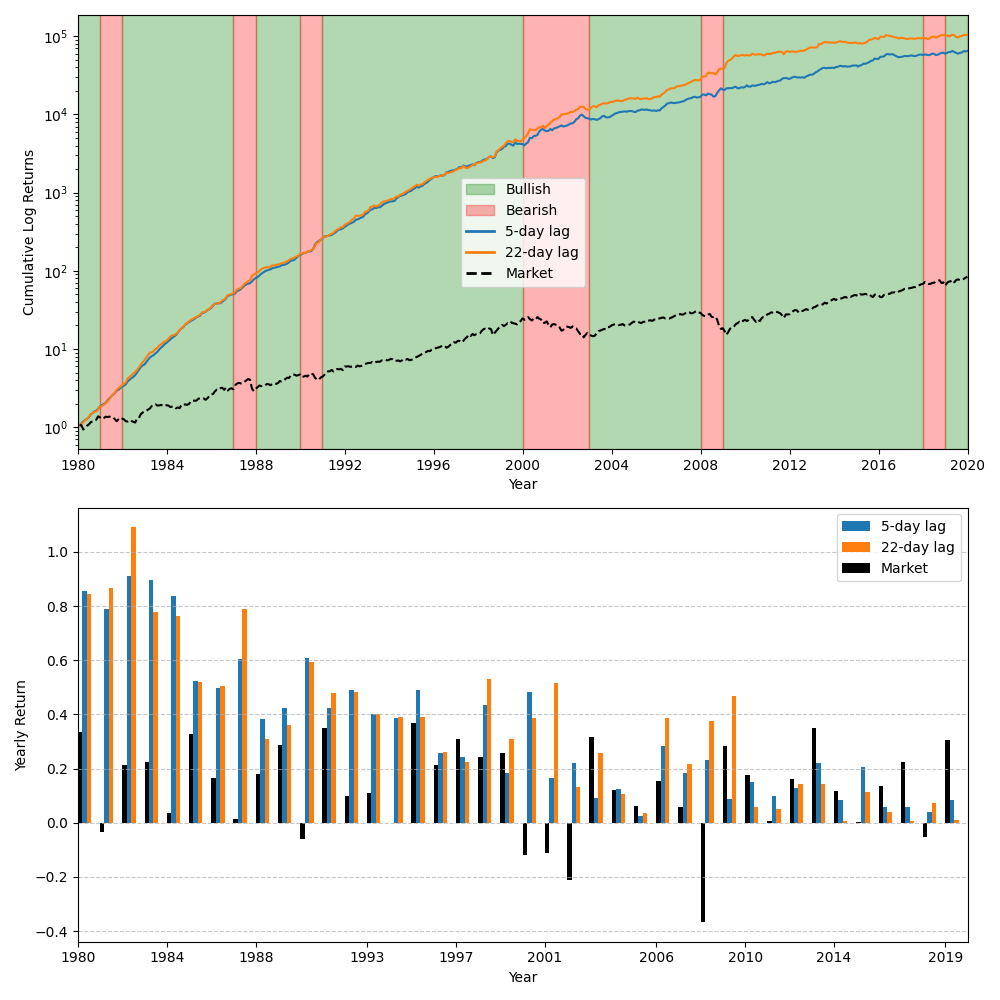
\includegraphics[width=0.8\textwidth]{2020_plot4_seq_len_comparison.png}
    \caption{Monthly cumulative returns and raw annual returns for prior week (5) and prior month (22) input data.}
    \label{fig:seq_len_comp}
\end{figure}

% 2020 table
\begin{table}[h]
    \centering
    \begin{tabular}{lcccccc}
        \toprule
        & Period & $\alpha$ & $\alpha$ (Annual) & $\beta$ & Sharpe Ratio \\
        \midrule
        \multirow{3}{*}{5-day lag} & 1980-1995 & 0.16* & 51.57 & 0.01 & 1.49 \\
                                   & 1995-2010 & 0.06* & 17.43 & 0.03 & 0.40 \\
                                   & 2010-2020 & 0.04* & 10.65 & 0.04 & 0.38 \\
        \midrule
        \multirow{3}{*}{22-day lag} & 1980-1995 & 0.16* & 51.73 & -0.00 & 1.34 \\
                                    & 1995-2010 & 0.09* & 26.99 & 0.01 & 0.55 \\
                                    & 2010-2020 & 0.02* & 5.66 & 0.05 & 0.20 \\
        \bottomrule
    \end{tabular}
    \caption{FF6 benchmark for varying day-lag input data. * signifies significant $\alpha$.}
    \label{tab:input_day_lag_comparison}
\end{table}

The comparison between models using 5-day and 22-day lag input data reveals interesting insights into their performance across different periods. In the first period (1980-1995), both configurations achieve significant alpha, with the 5-day lag model producing an annual alpha of 51.57\% and a Sharpe ratio of 1.49, while the 22-day lag model achieves an annual alpha of 51.73\% with a Sharpe ratio of 1.34. During the second period (1995-2010), the 5-day lag model shows an annual alpha of 17.43\% and a Sharpe ratio of 0.40, whereas the 22-day lag model outperforms with an annual alpha of 26.99\% and a Sharpe ratio of 0.55. However, in the third period (2010-2020), the performance of the 5-day lag model remains relatively strong with an annual alpha of 10.65\% and a Sharpe ratio of 0.38, while the 22-day lag model's performance drops to an annual alpha of 5.66\% and a Sharpe ratio of 0.20.

Given these results, the 5-day lag model is preferable, especially considering its superior performance in the most recent period (2010-2020). This period is crucial as it reflects the model's ability to adapt to more recent market dynamics and conditions. Additionally, the 5-day lag model consistently demonstrates better risk-adjusted returns as indicated by its higher Sharpe ratios across all periods, particularly in the 2010-2020 period. The higher Sharpe ratio indicates that the 5-day lag model provides better returns per unit of risk compared to the 22-day lag model. Therefore, despite the 22-day lag model's slightly better performance in the second period, the 5-day lag model's more consistent and robust performance, especially in recent years, makes it a more reliable choice for developing trading strategies.

% 2024 table
% \begin{table}[h]
%     \centering
%     \begin{tabular}{lcccccc}
%         \toprule
%         Model Type & Period & $\alpha$ & $\alpha$ (Annual) & $\beta$ & Sharpe Ratio \\
%         \midrule
%         \multirow{3}{*}{5-day lag} & 1980-1995 & 0.16* & 51.57 & 0.01 & 1.49 \\
%                                    & 1995-2010 & 0.06* & 17.43 & 0.03 & 0.40 \\
%                                    & 2010-2024 & 0.05* & 14.69 & 0.03 & 0.41 \\
%         \midrule
%         \multirow{3}{*}{22-day lag} & 1980-1995 & 0.16* & 51.73 & -0.00 & 1.34 \\
%                                     & 1995-2010 & 0.09* & 26.99 & 0.01 & 0.55 \\
%                                     & 2010-2024 & 0.03* & 8.38 & 0.06 & 0.25 \\
%         \bottomrule
%     \end{tabular}
%     \caption{Input Day Lag Comparison}
%     \label{tab:input_day_lag_comparison}
% \end{table}


\begin{figure}[H]
    \centering
    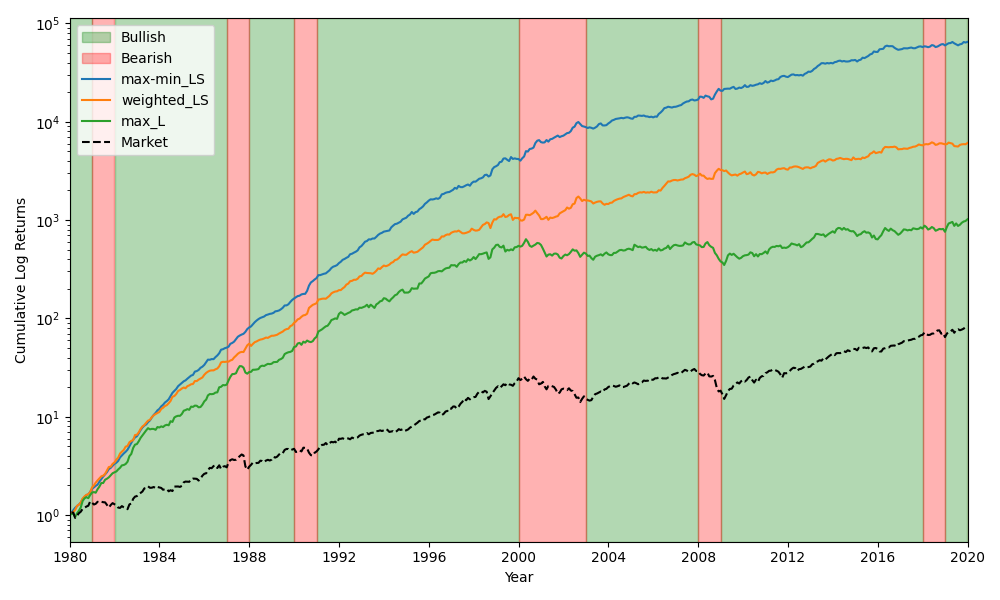
\includegraphics[width=0.9\textwidth]{2020_plot5_portfolio_strategy_comparison.png}
    \caption{Monthly cumulative returns for varying portfolio trading strategies.}
    \label{fig:strategy_comp}
\end{figure}

% 2020 table
\begin{table}[h]
    \centering
    \begin{tabular}{lcccccc}
        \toprule
        & Period & $\alpha$ & $\alpha$ (Annual) & $\beta$ & Sharpe Ratio \\
        \midrule
        \multirow{3}{*}{max-min Long-Short} & 1980-1995 & 0.16* & 51.57 & 0.01 & 1.49 \\
                                            & 1995-2010 & 0.06* & 17.43 & 0.03 & 0.40 \\
                                            & 2010-2020 & 0.04* & 10.65 & 0.04 & 0.38 \\
        \midrule
        \multirow{3}{*}{weighted Long-Short} & 1980-1995 & 0.13* & 42.38 & -0.05 & 1.00 \\
                                             & 1995-2010 & 0.03* & 9.44 & 0.04 & 0.20 \\
                                             & 2010-2020 & 0.03* & 7.28 & 0.08 & 0.25 \\
        \midrule
        \multirow{3}{*}{max Long} & 1980-1995 & 0.09* & 28.35 & 0.68 & 0.57 \\
                                  & 1995-2010 & -0.01* & -3.86 & 0.65 & 0.03 \\
                                  & 2010-2020 & -0.00 & -0.33 & 0.73 & 0.17 \\
        \bottomrule
    \end{tabular}
    \caption{FF6 benchmark for varying portfolio trading strategies. * signifies significant $\alpha$.}
    \label{tab:portfolio_strategy_comparison}
\end{table}


The comparison of portfolio trading strategies indicates that the Max-Min Long-Short (LS) strategy consistently performs the best across all periods. This strategy achieves significant alphas and the highest Sharpe ratios in each period. The primary reason for its superior performance is likely due to its method of trading based on the highest absolute value predicted returns. By going long on the top decile of industries with the highest predicted returns and shorting the bottom decile with the lowest predicted returns, the strategy effectively captures significant market movements and exploits both bullish and bearish opportunities, leading to more robust returns.

In contrast, the Weighted Long-Short (LS) strategy, while still profitable, does not perform as well because it weights positions proportionally to predicted returns, which may dilute the impact of extreme predictions and lead to less optimal allocation. This approach can result in less pronounced returns compared to the Max-Min LS strategy. The Max Long strategy, on the other hand, shows the highest beta and lower Sharpe ratios, indicating higher volatility and risk. This is because it only takes long positions on the single industry with the highest predicted return, without any hedging through short positions. This lack of diversification and risk management results in higher exposure to market fluctuations, leading to less stable and lower risk-adjusted returns.

% 2024 table
% \begin{table}[h]
%     \centering
%     \begin{tabular}{lcccccc}
%         \toprule
%         Model Type & Period & $\alpha$ & $\alpha$ (Annual) & $\beta$ & Sharpe Ratio \\
%         \midrule
%         \multirow{3}{*}{max-min Long-Short} & 1980-1995 & 0.16* & 51.57 & 0.01 & 1.49 \\
%                                             & 1995-2010 & 0.06* & 17.43 & 0.03 & 0.40 \\
%                                             & 2010-2024 & 0.05* & 14.69 & 0.03 & 0.41 \\
%         \midrule
%         \multirow{3}{*}{weighted Long-Short} & 1980-1995 & 0.13* & 42.38 & -0.05 & 1.00 \\
%                                              & 1995-2010 & 0.03* & 9.44 & 0.04 & 0.20 \\
%                                              & 2010-2024 & 0.03* & 9.43 & 0.07 & 0.27 \\
%         \midrule
%         \multirow{3}{*}{max Long} & 1980-1995 & 0.09* & 28.35 & 0.68 & 0.57 \\
%                                   & 1995-2010 & -0.01* & -3.86 & 0.65 & 0.03 \\
%                                   & 2010-2020 & 0.01 & 2.11 & 0.70 & 0.20 \\
%         \bottomrule
%     \end{tabular}
%     \caption{Portfolio Strategy Comparison}
%     \label{tab:portfolio_strategy_comparison}
% \end{table}


% \begin{figure}[H]
%     \centering
%     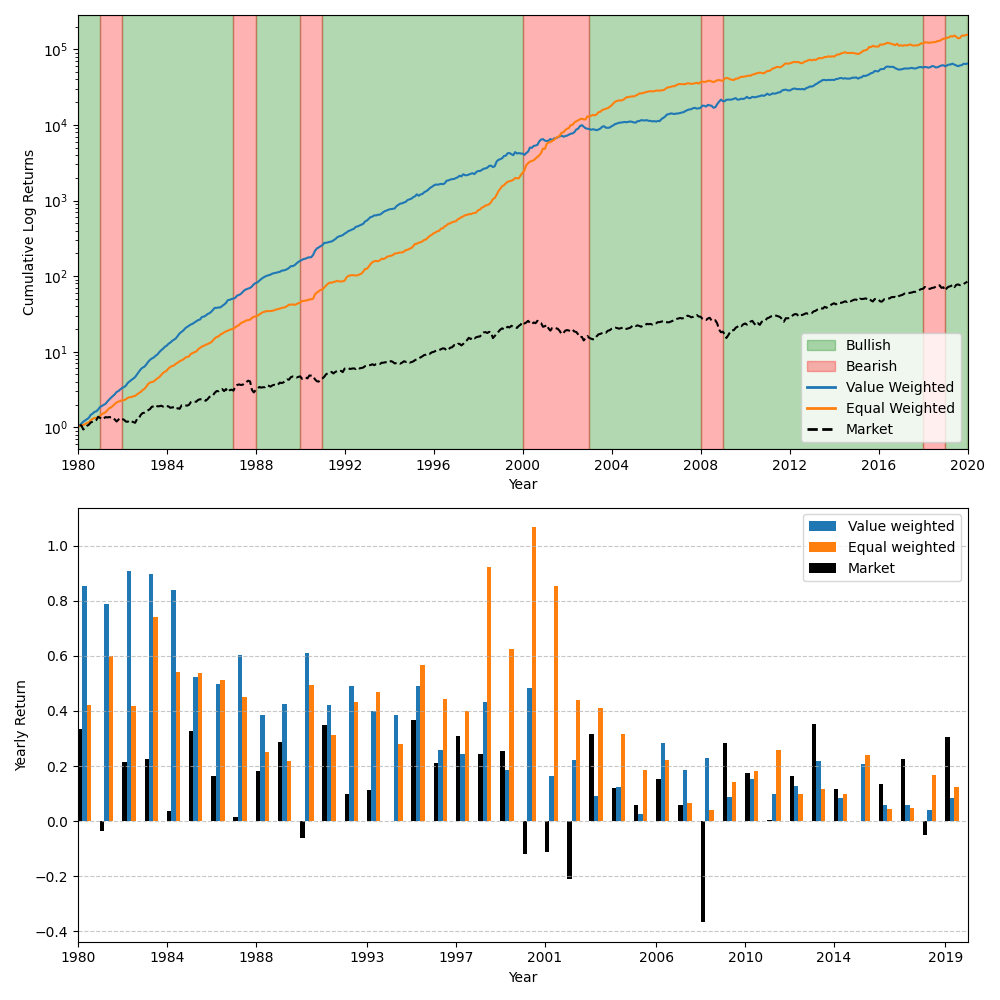
\includegraphics[width=0.8\textwidth]{2020_plot6_portfolio_weighting_comparison.png}
%     \caption{Monthly cumulative and raw annual returns for equal and value-weighted data.}
%     \label{fig:data_weighing_comp}
% \end{figure}

% % 2020 table
% \begin{table}[H]
%     \centering
%     \begin{tabular}{lcccccc}
%         \toprule
%         Model Type & Period & Alpha & Alpha (Annualized) & Beta & Sharpe Ratio \\
%         \midrule
%         \multirow{3}{*}{Value weighted} & 1980-1995 & 0.16* & 51.57 & 0.01 & 1.49
%         \\
%                                         & 1995-2010 & 0.06* & 17.43 & 0.03 & 0.40 \\
%                                         & 2010-2020 & 0.04* & 10.65 & 0.04 & 0.38 \\
%         \midrule
%         \multirow{3}{*}{Equal weighted} & 1980-1995 & 0.12* & 35.46 & 0.01 & 1.08 \\
%                                         & 1995-2010 & 0.13* & 39.2 & -0.04 & 0.79 \\
%                                         & 2010-2020 & 0.05* & 13.87 & -0.01 & 0.41 \\
%         \bottomrule
%     \end{tabular}
%     \caption{FF6 benchmark for equal and value weighted Fama French Industry Portfolios data. * signifies significant $\alpha$.}
%     \label{tab:data_weighing_comp}
% \end{table}

% % 2024 table
% % \begin{table}[h]
% %     \centering
% %     \begin{tabular}{lcccccc}
% %         \toprule
% %         Model Type & Period & Alpha & Alpha (Annualized) & Beta & Sharpe Ratio \\
% %         \midrule
% %         \multirow{3}{*}{Value weighted} & 1980-1995 & 0.16* & 51.57 & 0.01 & 1.49 \\
% %                                         & 1995-2010 & 0.06* & 17.43 & 0.03 & 0.40 \\
% %                                         & 2010-2024 & 0.05* & 14.69 & 0.03 & 0.41 \\
% %         \midrule
% %         \multirow{3}{*}{Equal weighted} & 1980-1995 & 0.12* & 35.46 & 0.01 & 1.08 \\
% %                                         & 1995-2010 & 0.13* & 39.2 & -0.04 & 0.79 \\
% %                                         & 2010-2024 & 0.06* & 17.46 & -0.01 & 0.45 \\
% %         \bottomrule
% %     \end{tabular}
% %     \caption{Industry Data Weighing Comparison}
% %     \label{tab:data_weighing_comp}
% % \end{table}



% % In Figure \ref{fig:data_weighing_comp}, the equal weighted industries data actually outperform our model. This is expected and can be explained by the Size Fama French factor which holds that large cap companies are overvalued compared to their smaller cap counterparts. The value weighted industries will not be able to capture this arbitrage opportunity, but we chose it regardless because in a real world scenario we may not be able to buy all stocks equally and it is risky to buy large quantities of a small cap stock at scale regardless of returns because of volume concerns. Additionally, ETFs are more likely to be found matching the value than equal portfolio which would make it easier  and more practical to trade this strategy. Even without ETFs, we would likely have higher transaction fees for the equal weighted portfolios because they would result in making more trades since they are buying more of small cap stocks to match the equity in large cap stocks.

% The results indicate that the equal-weighted portfolio strategy outperforms the value-weighted strategy in terms of both alpha and Sharpe ratio, particularly in the periods after 1995. For the period 1995-2010, the equal-weighted strategy achieves an annual alpha of 39.2\% and a Sharpe ratio of 0.79, compared to the value-weighted strategy's 17.43\% alpha and 0.40 Sharpe ratio. Similarly, in the period 2010-2020, the equal-weighted strategy continues to show superior performance with an annual alpha of 13.87\% and a Sharpe ratio of 0.41, while the value-weighted strategy generates an annual alpha of 10.65\% and a Sharpe ratio of 0.38. This consistent outperformance by the equal-weighted strategy can be attributed to its higher exposure to smaller-cap stocks, which tend to yield higher returns due to the size premium effect.

% Despite the higher returns, we still prefer the value-weighted strategy for practical reasons related to trading. In real-world scenarios, it is more challenging to trade equal-weighted portfolios because it requires buying and maintaining larger positions in smaller-cap stocks, which can be difficult due to volume constraints and increased market impact. Additionally, value-weighted portfolios align more closely with ETFs, making them easier and more cost-effective to trade. Even if not trading on ETFs but purely stocks by industry, frequent rebalancing needed to maintain equal weights in the portfolio also leads to higher transaction fees, which can erode net returns. The value-weighted strategy, though not capturing the full arbitrage opportunity presented by the size factor, offers a more practical and feasible approach for large-scale trading, providing stable and consistent returns with lower operational complexities and costs.

\medskip

\section{Discussion}
The results of our analysis show that machine learning models, particularly the Long Short-Term Memory (LSTM) networks, can effectively capture market trends and generate consistent positive returns across different market regimes.

% Our findings indicate that the LSTM model, when trained on value-weighted Fama French 49 Industry Portfolio Returns using a 5-day lag and applied through the Max-Min Long-Short strategy, produced the highest alpha. This model consistently generated significant positive returns across various market conditions, including both bullish and bearish periods. The robustness of this model is further highlighted by its low beta, indicating minimal correlation with market movements and demonstrating its ability to provide excess returns independent of overall market trends.

% The data emphasizes the superiority of the LSTM model for financial market predictions due to its ability to adapt and maintain high performance across different market regimes. The consistent alpha generation and favorable Sharpe ratios of the LSTM model highlight its effectiveness in capturing market trends and providing reliable risk-adjusted returns. In contrast, the more variable performance of the FFNN and GBDT models suggests that they may be less suited for long-term, dynamic market conditions, reinforcing the preference for LSTM in developing advanced trading strategies.

Our findings indicate that the LSTM model, when trained on value-weighted Fama French 49 Industry Portfolio Returns using a 5-day lag and applied through the Max-Min Long-Short strategy, produced the highest alpha. This model consistently generated significant positive returns across various market conditions, including both bullish and bearish periods. For example, the LSTM model achieved an annual alpha of 51.57\% during 1980-1995, 17.43\% during 1995-2010, and 10.65\% during 2010-2020. The robustness of this model is further highlighted by its low beta values, indicating minimal correlation with market movements and demonstrating its ability to provide excess returns independent of overall market trends.

The data emphasizes the superiority of the LSTM model for financial market predictions due to its ability to adapt and maintain high performance across different market regimes. The consistent alpha generation and favorable Sharpe ratios of the LSTM model highlight its effectiveness in capturing market trends and providing reliable risk-adjusted returns. In contrast, the more variable performance of the FFNN and GBDT models suggests that they may be less suited for long-term, dynamic market conditions, reinforcing the preference for LSTM in developing advanced trading strategies. For instance, the Sharpe ratios for the LSTM model were 1.49, 0.40, and 0.38 across the three periods, respectively.

Moreover, our analysis across different market periods reveals that the model’s performance remains strong, though it exhibits a decline in alpha over time. This decline may be attributed to the increasing prevalence of machine learning for market analysis and prediction and the overall AI boom in the late 2010s.

Our study also underscores the importance of model configuration and parameter selection. The number of industries, input day lags, portfolio strategy type, and industry data weighting significantly impact model performance. For instance, models trained on a larger number of industries (e.g., 49 industries) generally outperformed those trained on fewer industries (e.g., 5 industries) due to increased diversification. In fact, from Figure \ref{fig:industry_comp} the lower industry models taper off and end up with little to no returns in latter years, likely because of their simplicity being factored in to the market. 

Interestingly, there does not seem to be a significant difference between the number of Day Lags as seen in Table \ref{tab:input_day_lag_comparison}. We experimented with a 1 Day Lag (not included in results) which performed worse than both current models, but the similarity between the weekly (5 Day) and monthly (22 Day) Lags could mean that the models can learn sufficiently well using only the past week's worth of data.

As seen in Figure \ref{fig:strategy_comp}, our chosen portfolio strategy of Max-Min Long Short was also important to model performance. By choosing to invest only in the top and bottom deciles, we minimize our exposure to uncertainty by choosing to short or long industries that are particularly well or poorly, respectively.

\medskip

\subsection{Future Research and Limitations}

\subsubsection{\emph{Future Research}}
% In the future, we would like to implement the following changes to our models to
% improve their performance and robustness:
% \begin{itemize}
%     \item \textbf{Temporal Data Weighing}: Since more recent market data is
%     likely to be more critical to predicting future returns, we hypothesize that
%     weighing recent data more heavily will result in a model with better
%     predictive power.
%     \item \textbf{Class Imbalance Handling}: Since the market tends to go up
%     over time, it is reasonable to assume that there is a bias in the returns
%     for each industry to be positive. Interestingly, the best models that we
%     found typically differentiated themselves by being able to outperform the
%     market (typically by shorting industries that were predicted to have
%     negative returns) rather than by being able to predict the industries that
%     would have the highest returns. We could try to balance the classes in our
%     models to see if this improves our models' performance.
%     \item \textbf{New Features}: We could try introducing new features into our
%     model inputs such as information about industry-wide earnings data, news
%     sentiment, and technical indicators such as moving averages, Relative
%     Strength Index (RSI), and Moving Average Convergence/Divergence (MACD).

% \end{itemize}

In future research, we aim to implement several enhancements to improve our models' performance and robustness. (1) temporal data weighting. By giving more weight to recent market data in the training process of each model, we hypothesize that the models will have better predictive power, as more recent information is likely to be more relevant for future returns. (2) class imbalance handling. Given the market's tendency to rise over time, there is a bias in returns for each industry to be positive. By balancing the classes in our models, we could potentially improve their prediction abilities. (3) new input features, such as industry-wide earnings data, news sentiment, and technical indicators like moving averages, Relative Strength Index (RSI), and Moving Average Convergence/Divergence (MACD). 



% \subsubsection{Limitations}
% \begin{itemize}
%     \item \textbf{Transaction Fees}: We do not account for transaction fees in
%     our backtest which can significantly affect the performance of our models.
%     Though we find that the 49 industry models tend to outperform the 10
%     industry models, the 49 industry models have more transactions and thus may
%     ultimately perform worse when accounting for transaction fees.
%     \item \textbf{Model Trained Yearly}: We train our model yearly but it is
%     likely that as we approach the current year our model's performance will
%     degrade as machine learning models are continually accounted for in market
%     returns. In order to counteract this, we could train our model on a rolling
%     monthly rather than yearly basis and likely achieve higher returns.
%     \item \textbf{Tradability}: Though we use the Fama French Industry
%     Portfolios as a proxy for trading, in reality we would have to find ETFs to
%     trade which may not perfectly reflect the industry returns and thus reduce
%     our model's predictive power.
%     \item \textbf{No Regularization}: Currently, we do not incorporate any
%     checks on our model's outputs. This is to say, if the model predicts that a
%     single industry will have a return of 1000\%, we will invest all our money
%     in that industry which could be disastrous and risky. We could incorporate
%     stop losses or reweights/resampling on model predictions to prevent
%     this.
%     \item \textbf{Insensitivity to Intraday Data}: We only use daily data in our
%     models which means that we are exposed to overnight or intraday risk. In the
%     course of a day, important market announcements requiring quick buys or,
%     more importantly, sells could be made which our model would not be able to
%     account for.
% \end{itemize}

\subsubsection{\emph{Risks and Limitations}}
There are several limitations to our study that must be acknowledged. (1) transaction fees were not accounted for in our backtest, which will lower the alpha for higher industry count portfolios. (2) we trained our models on a yearly basis, but since this is a daily strategy it would be most accurate to train daily to get most accurate alphas. (3) while we used the Fama French Industry Portfolios as a proxy for trading, actual implementation would require finding ETFs to trade, which may not perfectly reflect industry returns and could reduce the models' predictive power. (4) we did not incorporate any regularization checks on our models' outputs. This means that if a model predicts an extraordinarily high return for a single industry, it could lead to disproportionate investments in that industry, posing significant risks. Implementing stop losses or reweighting/resampling model predictions could mitigate this issue. (4) our models were insensitive to intraday data, relying solely on daily data. This exposure to overnight or intraday risk means that our models may not react promptly to significant market announcements requiring immediate buys or sells. Addressing these limitations will be crucial for translating our models' theoretical success into practical, real-world trading strategies.

\medskip

\medskip

\section{Conclusion}
% We find that our models are able to generate positive and significant alpha
% relative to the FF6 factors benchmark and that they are also uncorrelated with
% them ($\beta$ close to 0). In particular, we find that the LSTM model is able to
% capture market trends in the 49 industry Fama French portfolios and generate
% consistent positive returns across different market regimes. We also find that
% the 49 industry models tend to outperform the 10 industry models potentially
% because of their increased diversification. We also found that the 22 and 5 day
% lags tended to perform similarly across various models. Our findings suggest
% that if we were able to implement our models in a real-world scenario, we would
% expect to generate consistent alpha and outperform the market but there are some
% hurdles to this such as transaction fees and whether the Fama French Industry
% Portfolios are able to be traded through appropriate ETFs.

% In summary, our research demonstrates the potential of advanced machine learning models to enhance trading strategies and deliver superior returns in financial markets. By rigorously evaluating different models and configurations, we provide valuable insights into the factors that contribute to successful trading strategies based on the Fama French Industry Portfolios. However, practical implementation challenges, such as transaction fees and the tradability of these portfolios through ETFs, must be addressed to fully realize the benefits of these models in real-world trading scenarios.

% Our research demonstrates that advanced machine learning models, particularly LSTM networks, have significant potential to enhance trading strategies and deliver superior returns in financial markets. By rigorously evaluating different models and configurations, we identified the LSTM model trained on value-weighted Fama French 49 Industry Portfolio Returns using a 5-day lag and applied through the Max-Min Long-Short strategy as the most effective. This configuration consistently generated significant positive returns, with low beta indicating minimal correlation with market movements, thus providing excess returns independent of overall market trends. Our findings also emphasize the importance of model configuration and parameter selection. Models trained on a larger number of industries (e.g., 49 industries) generally outperformed those trained on fewer industries, due to increased diversification. Additionally, our chosen portfolio strategy of Max-Min Long-Short was crucial to model performance, effectively capturing significant market movements and exploiting both bullish and bearish opportunities. While the LSTM model showed robustness across different market periods (1980-1995, 1996-2010, and 2011-2020), we observed a decline in alpha over time. This trend may be attributed to the increasing prevalence of machine learning in market analysis and the overall AI boom in the late 2010s. Despite this, the LSTM model remained the best performer, demonstrating superior adaptability and consistent risk-adjusted returns compared to FFNN and GBDT models. 

Our research demonstrates that machine learning models, especially Long Short-Term Memory (LSTM) networks, can effectively capture market trends and generate consistent positive returns across different market regimes. The LSTM model, trained on value-weighted Fama French 49 Industry Portfolio Returns using a 5-day lag and applied through the Max-Min Long-Short strategy, produced the highest alpha. Specifically, this model achieved significant annual alphas of 51.57\% during the period from 1980 to 1995, 17.43\% from 1995 to 2010, and 10.65\% from 2010 to 2020. These results highlight the model's ability to generate excess returns independent of overall market movements, as indicated by its consistently low beta values near zero.

The robustness of the LSTM model is further evidenced by its high Sharpe ratios, which measure the risk-adjusted returns. The Sharpe ratios were 1.49 for the period 1980-1995, 0.40 for 1995-2010, and 0.38 for 2010-2020, underscoring the model's effectiveness in providing reliable returns with manageable risk. The comparative analysis showed that the LSTM model outperformed other architectures, such as Feed Forward Neural Networks (FFNN) and Gradient Boosting Decision Trees (GBDT), which exhibited more variable performance and lower Sharpe ratios.

Moreover, our analysis across different market periods revealed that while the LSTM model's alpha declined over time, it remained significant, reflecting the model's adaptability to changing market conditions. The number of industries included in the model also played a crucial role, with the 49-industry configuration consistently outperforming those with fewer industries due to increased diversification. Further, the 22-day lag did for all data before 2010 but after the 5-day lag did better.

Our chosen portfolio strategy, the Max-Min Long-Short, proved to be the most effective, leveraging the highest and lowest predicted returns to maximize gains and minimize risks. This strategy consistently yielded higher alphas and Sharpe ratios compared to the Weighted Long-Short and Max Long strategies.
 
In terms of future research, we propose several enhancements to improve model performance and robustness, including temporal data weighting, class imbalance handling, and the introduction of new features such as industry-wide earnings data, news sentiment, and technical indicators. These additions may provide a more comprehensive understanding of market dynamics, leading to more accurate predictions. We also acknowledge several limitations in our study, such as the exclusion of transaction fees, the need for more frequent model training, the practical challenges of trading Fama French Industry Portfolios through ETFs, the lack of regularization checks on model outputs, and the insensitivity to intraday data. Addressing these limitations will be crucial for translating our models' theoretical success into practical, real-world trading strategies.

\medskip

\bibliographystyle{plain}
\bibliography{references.bib}

\section{Appendix}

Redo of all results but with data up to 2024. The final plots and tables are for a comparison of equal-weighted and value-weighted industry portfolios.

\begin{figure}[H]
    \centering
    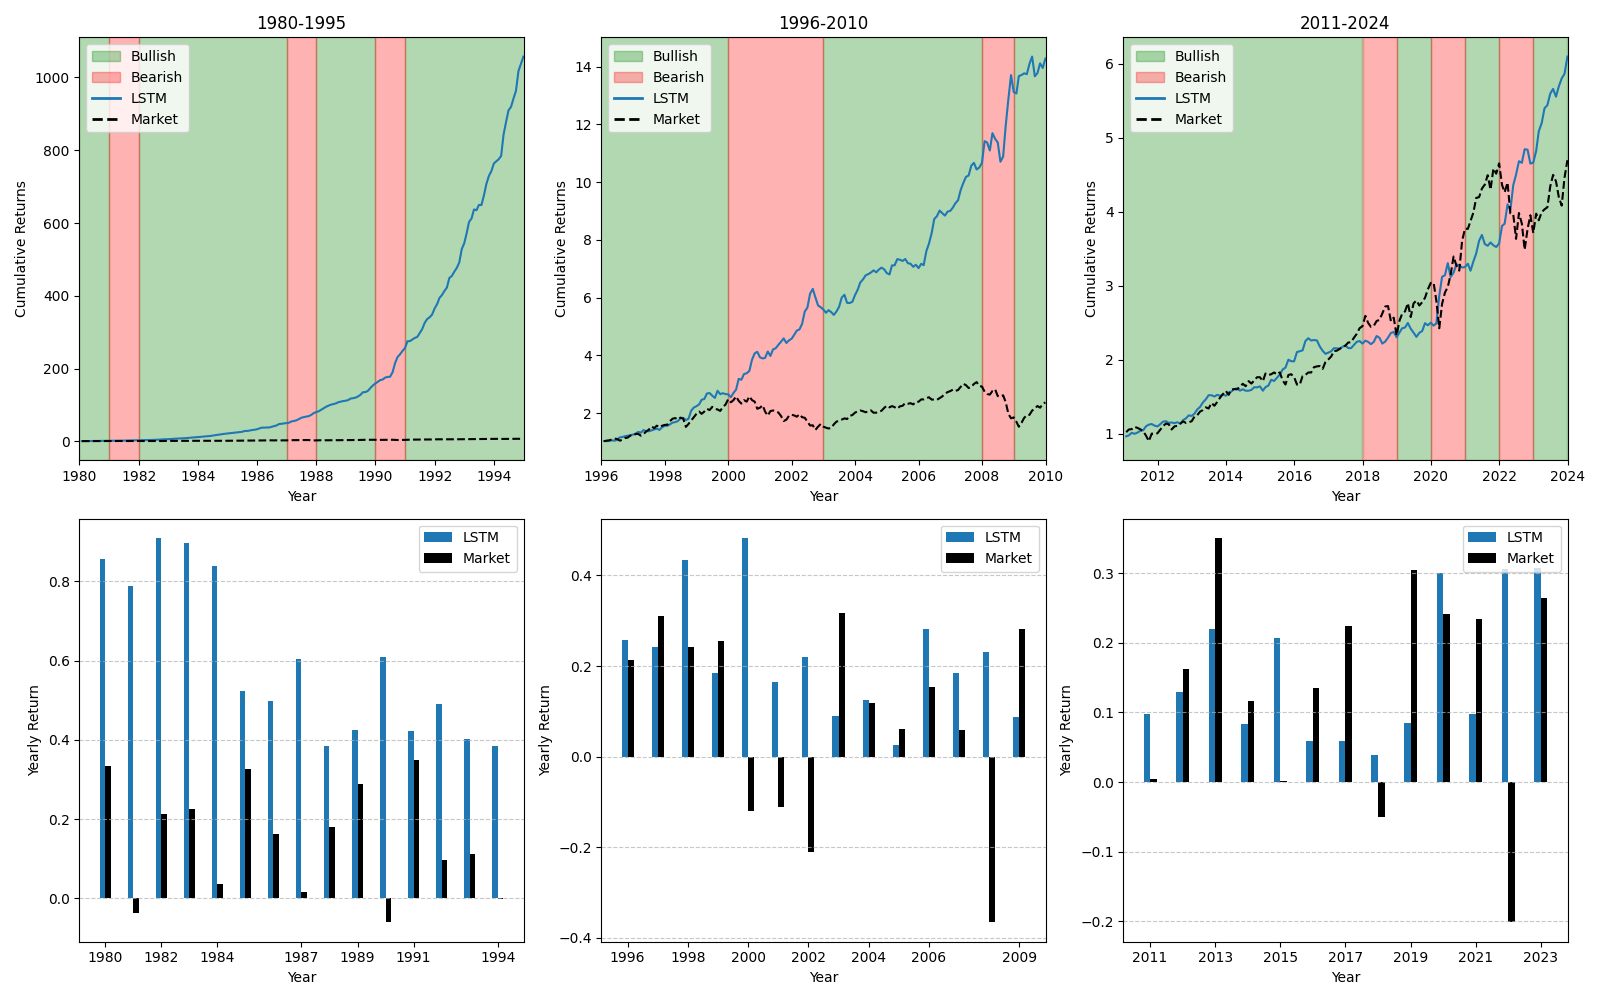
\includegraphics[width=0.8\textwidth]{2024_plot2_model_comparison_timeperiods.png}
    \caption{Monthly cumulative returns and annualized raw returns of best strategy in three separate time periods for data up to 2024.}
    \vspace{-10pt}
    \label{fig:timeperiods}
\end{figure}


\begin{table}[h]
    \centering
    \begin{minipage}{0.4\textwidth}
        \centering
        \begin{tabular}{lcccc}
            \toprule
            & $\alpha$ (Annual) & $\beta$ & Sharpe Ratio \\
            \midrule
            CAPM & 0.09* (28.18) & 0.01 & 0.65 \\
            FF3  & 0.09* (27.00) & 0.01 & 0.65 \\
            FF6  & 0.09* (27.47) & 0.02 & 0.65 \\
            \bottomrule
        \end{tabular}
        \caption{Best strategy CAPM, FF3, and FF6 benchmarks. $\alpha$ is daily and in percent. * signifies significant $\alpha$.}
        \label{tab:benchmarks}
    \end{minipage}
    \hspace{0.05\textwidth} % Adjust space between tables
    \begin{minipage}{0.4\textwidth}
        \centering
        \begin{tabular}{lcccc}
            \toprule
             & Period & $\alpha$ (Annual) & $\beta$ & Sharpe Ratio \\
            \midrule
            \multirow{3}{*}{Total} & 1980-1995 & 0.16* (51.57) & 0.01 & 1.49 \\
                                   & 1995-2010 & 0.06* (17.43) & 0.03 & 0.40 \\
                                   & 2010-2024 & 0.05* (14.69) & 0.03 & 0.41 \\
            \midrule
            \multirow{3}{*}{Bullish} & 1980-1995 & 0.15* (50.32) & -0.00 & 1.05 \\
                                     & 1995-2010 & 0.05* (15.36) & 0.03 & 0.33 \\
                                     & 2010-2024 & 0.04* (12.37) & 0.04 & 0.38 \\
            \midrule
            \multirow{3}{*}{Bearish} & 1980-1995 & 0.17* (58.5) & 0 & 0.45 \\
                                     & 1995-2010 & 0.07* (21.03) & 0.02 & 0.26 \\
                                     & 2010-2014 & 0.07* (21.07) & 0.03 & 0.29 \\
            \bottomrule
        \end{tabular}
    \end{minipage}
\end{table}

\newpage

\begin{figure}[H]
    \centering
    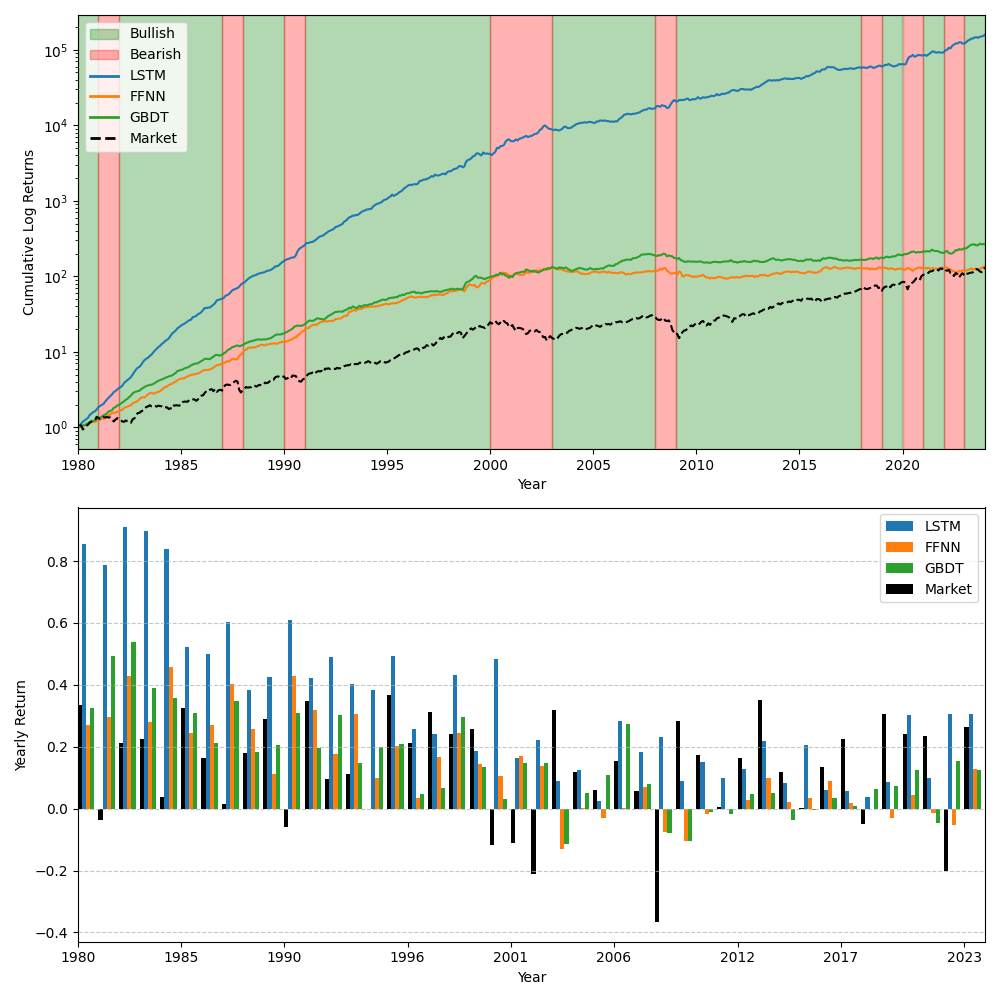
\includegraphics[width=0.9\textwidth]{2024_plot1_model_comparison.png}
    \caption{Monthly cumulative returns and raw annual returns for varying model types for data up to 2024.}
    \label{fig:model_comp}
\end{figure}

% 2024 table
\begin{table}[h]
    \centering
    \begin{tabular}{lcccccc}
        \toprule
        & Period & $\alpha$ (Annual) & $\beta$ & Sharpe Ratio \\
        \midrule
        \multirow{3}{*}{LSTM} & 1980-1995 & 0.16* (51.57) & 0.01 & 1.49 \\
                              & 1995-2010 & 0.06* (17.43) & 0.03 & 0.40 \\
                              & 2010-2024 & 0.05* (14.69) & 0.03 & 0.41 \\
        \midrule
        \multirow{3}{*}{FFNN} & 1980-1995 & 0.07* (20.70) & -0.04 & 0.70 \\
                              & 1995-2010 & 0.01 (1.60) & 0.01 & 0.05 \\
                              & 2010-2024 & 0.01* (3.31) & -0.08 & 0.08 \\
        \midrule
        \multirow{3}{*}{GBDT} & 1980-1995 & 0.07* (21.38) & 0.05 & 0.80 \\
                              & 1995-2010 & 0.02* (4.49) & 0.01 & 0.12 \\
                              & 2010-2024 & 0.01* (3.23) & 0.03 & 0.14 \\
        \bottomrule
    \end{tabular}
    \caption{Model Architecture Comparison}
    \label{tab:model_comp}
\end{table}

\newpage

\begin{figure}[H]
    \centering
    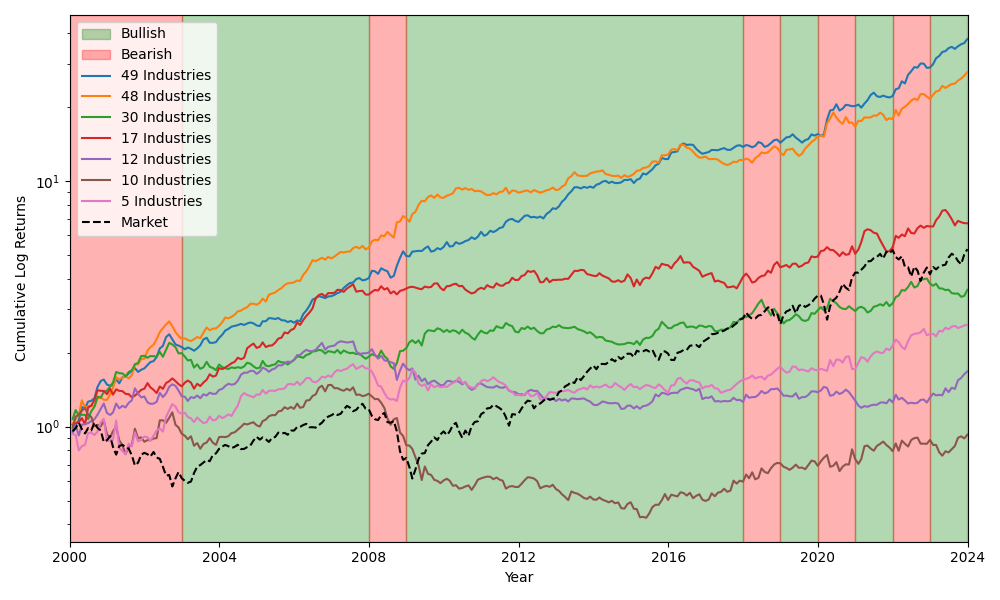
\includegraphics[width=0.7\textwidth]{2024_plot3_num_industries_comparison.png}
    \caption{Monthly cumulative returns for varying number of industries for data up to 2024.}
    \label{fig:industry_comp}
\end{figure}

\begin{table}[h]
    \centering
    \begin{tabular}{lcccccc}
        \toprule
        & Period & $\alpha$ & $\alpha$ (Annual) & $\beta$ & Sharpe Ratio \\
        \midrule
        \multirow{3}{*}{49 Industries} & 1980-1995 & 0.16* & 51.57 & 0.01 & 1.49 \\
                                       & 1995-2010 & 0.06* & 17.43 & 0.03 & 0.40 \\
                                       & 2010-2024 & 0.05* & 14.69 & 0.03 & 0.41 \\
        \midrule
        \multirow{3}{*}{48 Industries} & 1980-1995 & 0.16* & 53.09 & 0.02 & 1.37 \\
                                       & 1995-2010 & 0.08* & 23.28 & 0.02 & 0.48 \\
                                       & 2010-2024 & 0.03* & 8.8 & 0.01 & 0.24 \\
        \midrule
        \multirow{3}{*}{30 Industries} & 1980-1995 & 0.12* & 39.05 & 0.02 & 1.17 \\
                                       & 1995-2010 & 0.04* & 10.07 & -0.02 & 0.21 \\
                                       & 2010-2024 & 0.01* & 3.06 & -0.02 & 0.07 \\
        \midrule
        \multirow{3}{*}{17 Industries} & 1980-1995 & 0.18* & 58.77 & -0.03 & 1.29 \\
                                       & 1995-2010 & 0.08* & 21.97 & -0.03 & 0.40 \\
                                       & 2010-2024 & 0.02* & 5.31 & -0.02 & 0.11 \\
        \midrule
        \multirow{3}{*}{12 Industries} & 1980-1995 & 0.19* & 63.97 & -0.05 & 1.43 \\
                                       & 1995-2010 & 0.03* & 8.76 & -0.01 & 0.19 \\
                                       & 2010-2024 & 0.00 & 0.8 & -0.04 & 0.01 \\
        \midrule
        \multirow{3}{*}{10 Industries} & 1980-1995 & 0.24* & 88.93 & -0.06 & 1.36 \\
                                       & 1995-2010 & -0.00 & -0.39 & -0.05 & 0.01 \\
                                       & 2010-2024 & 0.02* & 4.43 & -0.04 & 0.07 \\
        \midrule
        \multirow{3}{*}{5 Industries} & 1980-1995 & 0.1* & 29.82 & -0.05 & 0.75 \\
                                      & 1995-2010 & 0.00 & 1.3 & 0.01 & 0.03 \\
                                      & 2010-2024 & 0.02* & 4.28 & -0.03 & 0.10 \\
        \bottomrule
    \end{tabular}
    \caption{FF6 benchmark for varying number of industries in different time periods. * signifies significant $\alpha$.}
    \label{tab:number_of_industries_comparison}
\end{table}

\newpage

\begin{figure}[H]
    \centering
    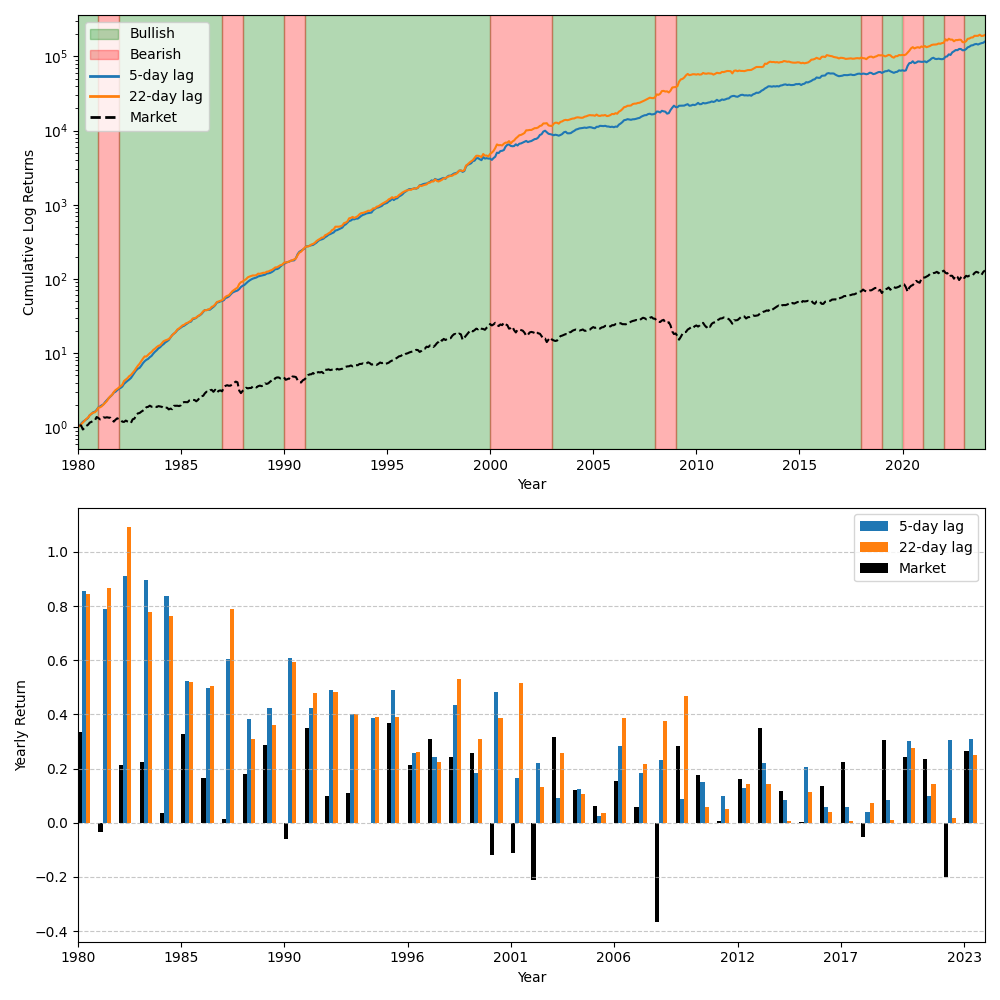
\includegraphics[width=0.8\textwidth]{2024_plot4_seq_len_comparison.png}
    \caption{Monthly cumulative returns and raw annual returns for prior week (5) and prior month (22) input data up to 2024.}
    \label{fig:seq_len_comp}
\end{figure}

\begin{table}[h]
    \centering
    \begin{tabular}{lcccccc}
        \toprule
        & Period & $\alpha$ & $\alpha$ (Annual) & $\beta$ & Sharpe Ratio \\
        \midrule
        \multirow{3}{*}{5-day lag} & 1980-1995 & 0.16* & 51.57 & 0.01 & 1.49 \\
                                   & 1995-2010 & 0.06* & 17.43 & 0.03 & 0.40 \\
                                   & 2010-2024 & 0.05* & 14.69 & 0.03 & 0.41 \\
        \midrule
        \multirow{3}{*}{22-day lag} & 1980-1995 & 0.16* & 51.73 & -0.00 & 1.34 \\
                                    & 1995-2010 & 0.09* & 26.99 & 0.01 & 0.55 \\
                                    & 2010-2024 & 0.03* & 8.38 & 0.06 & 0.25 \\
        \bottomrule
    \end{tabular}
    \caption{FF6 benchmark for varying day-lag input data. * signifies significant $\alpha$.}
    \label{tab:input_day_lag_comparison}
\end{table}

\begin{figure}[H]
    \centering
    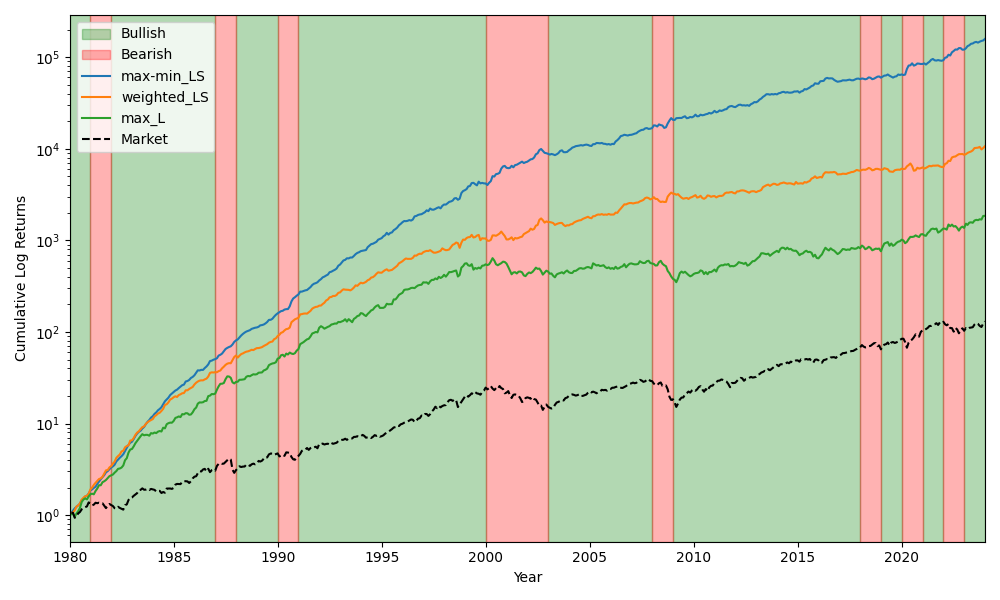
\includegraphics[width=0.9\textwidth]{2024_plot5_portfolio_strategy_comparison.png}
    \caption{Monthly cumulative returns for varying portfolio trading strategies for data up to 2024.}
    \label{fig:strategy_comp}
\end{figure}

\begin{table}[h]
    \centering
    \begin{tabular}{lcccccc}
        \toprule
        & Period & $\alpha$ & $\alpha$ (Annual) & $\beta$ & Sharpe Ratio \\
        \midrule
        \multirow{3}{*}{max-min Long-Short} & 1980-1995 & 0.16* & 51.57 & 0.01 & 1.49 \\
                                            & 1995-2010 & 0.06* & 17.43 & 0.03 & 0.40 \\
                                            & 2010-2024 & 0.05* & 14.69 & 0.03 & 0.41 \\
        \midrule
        \multirow{3}{*}{weighted Long-Short} & 1980-1995 & 0.13* & 42.38 & -0.05 & 1.00 \\
                                             & 1995-2010 & 0.03* & 9.44 & 0.04 & 0.20 \\
                                             & 2010-2024 & 0.03* & 9.43 & 0.07 & 0.27 \\
        \midrule
        \multirow{3}{*}{max Long} & 1980-1995 & 0.09* & 28.35 & 0.68 & 0.57 \\
                                  & 1995-2010 & -0.01* & -3.86 & 0.65 & 0.03 \\
                                  & 2010-2020 & 0.01 & 2.11 & 0.70 & 0.20 \\
        \bottomrule
    \end{tabular}
    \caption{FF6 benchmark for varying portfolio trading strategies. * signifies significant $\alpha$.}
    \label{tab:portfolio_strategy_comparison}
\end{table}

\newpage

\begin{figure}[H]
    \centering
    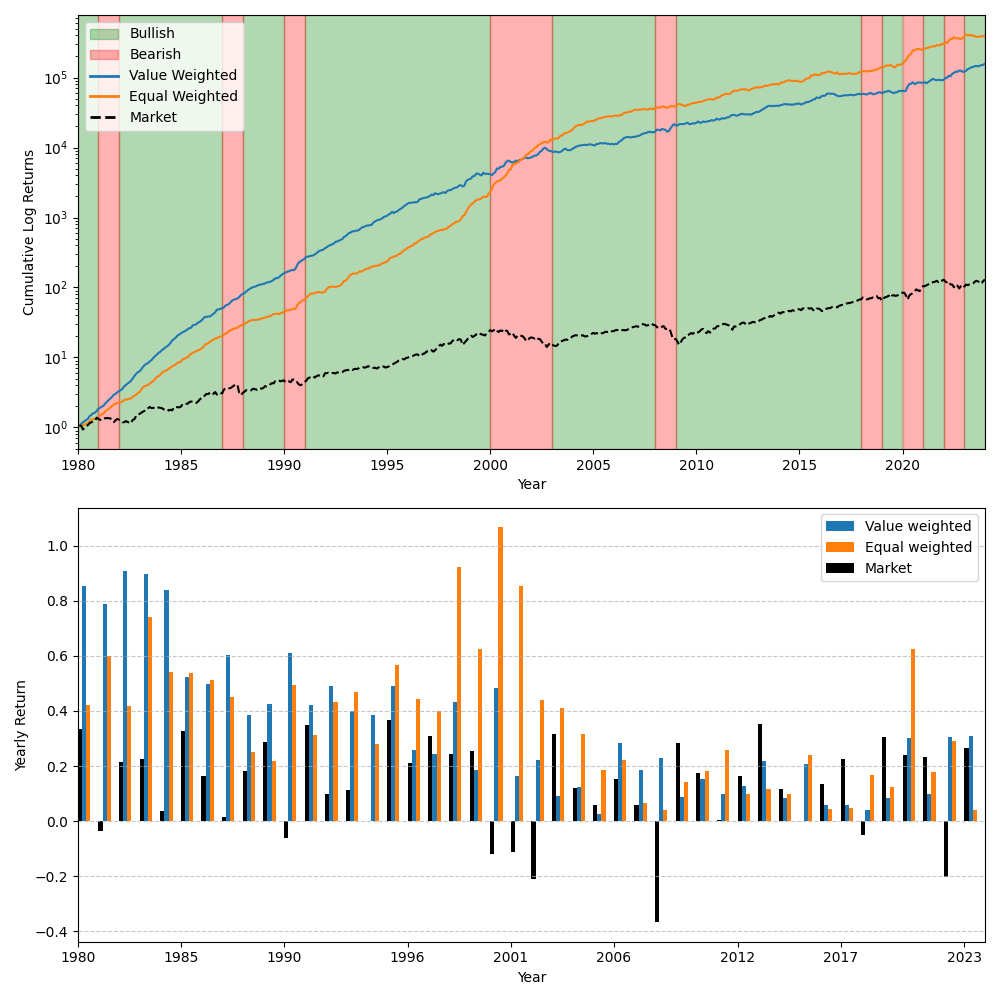
\includegraphics[width=0.8\textwidth]{2024_plot6_portfolio_weighting_comparison.png}
    \caption{Monthly cumulative and raw annual returns for equal and value-weighted data.}
    \label{fig:data_weighing_comp}
\end{figure}


% 2024 table
\begin{table}[h]
    \centering
    \begin{tabular}{lcccccc}
        \toprule
        & Period & Alpha & Alpha (Annualized) & Beta & Sharpe Ratio \\
        \midrule
        \multirow{3}{*}{Value weighted} & 1980-1995 & 0.16* & 51.57 & 0.01 & 1.49 \\
                                        & 1995-2010 & 0.06* & 17.43 & 0.03 & 0.40 \\
                                        & 2010-2024 & 0.05* & 14.69 & 0.03 & 0.41 \\
        \midrule
        \multirow{3}{*}{Equal weighted} & 1980-1995 & 0.12* & 35.46 & 0.01 & 1.08 \\
                                        & 1995-2010 & 0.13* & 39.2 & -0.04 & 0.79 \\
                                        & 2010-2024 & 0.06* & 17.46 & -0.01 & 0.45 \\
        \bottomrule
    \end{tabular}
    \caption{Industry Data Weighing Comparison}
    \label{tab:data_weighing_comp}
\end{table}



In Figure \ref{fig:data_weighing_comp}, the equal weighted industries data actually outperforms our model. This is expected and can be explained by the SMB (Small Minus Big) Fama French factor which holds that large cap companies are overvalued compared to their smaller cap counterparts. The value weighted industries will not be able to capture this arbitrage opportunity, but we chose it regardless because in a real world scenario we may not be able to buy all stocks equally and it is risky to buy large quantities of a small cap stock at scale regardless of returns because of volume concerns. Additionally, ETFs are more likely to be found matching the value than equal portfolio which would make it easier  and more practical to trade this strategy. Even without ETFs, we would likely have higher transaction fees for the equal weighted portfolios because they would result in making more trades since they are buying more of small cap stocks to match the equity in large cap stocks. For more information about why we chose value against equal weighted Industry data, refer to the bottom of the appendix.

The results indicate that the equal-weighted portfolio strategy outperforms the value-weighted strategy in terms of both alpha and Sharpe ratio, particularly in the periods after 1995. For the period 1995-2010, the equal-weighted strategy achieves an annual alpha of 39.2\% and a Sharpe ratio of 0.79, compared to the value-weighted strategy's 17.43\% alpha and 0.40 Sharpe ratio. Similarly, in the period 2010-2020, the equal-weighted strategy continues to show superior performance with an annual alpha of 13.87\% and a Sharpe ratio of 0.41, while the value-weighted strategy generates an annual alpha of 10.65\% and a Sharpe ratio of 0.38. This consistent outperformance by the equal-weighted strategy can be attributed to its higher exposure to smaller-cap stocks, which tend to yield higher returns due to the size premium effect.

Despite the higher returns, we still prefer the value-weighted strategy for practical reasons related to trading. In real-world scenarios, it is more challenging to trade equal-weighted portfolios because it requires buying and maintaining larger positions in smaller-cap stocks, which can be difficult due to volume constraints and increased market impact. Additionally, value-weighted portfolios align more closely with ETFs, making them easier and more cost-effective to trade. Even if not trading on ETFs but purely stocks by industry, frequent rebalancing needed to maintain equal weights in the portfolio also leads to higher transaction fees, which can erode net returns. The value-weighted strategy, though not capturing the full arbitrage opportunity presented by the size factor, offers a more practical and feasible approach for large-scale trading, providing stable and consistent returns with lower operational complexities and costs.

\end{document}